% Source PDF page 411 (printed p. 397)
\chapter{几何问题}
\section{在集合上的投影}
点 $x_0\in\R^n$ 到闭集 $C\subseteq\R^n$ 在范数 $\norm{\cdot}$ 下的距离定义为
\[\dist(x_0,C)=\inf\{\norm{x_0-x}\mid x\in C\}.\]
这里的下确界总能取到。把任意离 $x_0$ 最近的点 $z\in C$，即满足 $\norm{z-x_0}=\dist(x_0,C)$ 的点，称为 $x_0$ 在 $C$ 上的一个投影。一般而言，$x_0$ 在 $C$ 上可以有多个投影，即 $C$ 中可以有多个点离 $x_0$ 最近。

在一些特殊情况下，可以证明点在集合上的投影唯一。例如，若 $C$ 闭且凸，范数严格凸（例如欧氏范数），则对任意 $x_0$，总恰好存在一个离 $x_0$ 最近的 $z\in C$。一个有趣的逆命题是：若对每个 $x_0$，它在 $C$ 上的欧氏投影都唯一，则 $C$ 闭且凸，见习题8.2。

用 $P_C:\R^n\to\R^n$ 表示任意满足 $P_C(x_0)$ 是 $x_0$ 在 $C$ 上投影的函数，即对所有 $x_0$ 有
\[P_C(x_0)\in C,\qquad\norm{x_0-P_C(x_0)}=\dist(x_0,C).\]
换句话说，
\[P_C(x_0)=\argmin\{\norm{x-x_0}\mid x\in C\}.\]
称 $P_C$ 为在 $C$ 上的投影。
\begin{origexample}{8.1}
\textbf{在 $\R^2$ 的单位正方形上的投影。}考虑 $\R^2$ 中单位正方形的边界，即 $C=\{x\in\R^2\mid\norm x_\infty=1\}$，取 $x_0=0$。

在 $\ell_1$ 范数下，四个点 $(1,0),(0,-1),(-1,0),(0,1)$ 离 $x_0=0$ 最近，距离为一，因此 $\ell_1$ 范数下 $\dist(x_0,C)=1$。$\ell_2$ 范数下结论相同。

在 $\ell_\infty$ 范数下，$C$ 中所有点与 $x_0$ 的距离都为一，$\dist(x_0,C)=1$。
\end{origexample}
% Source PDF page 412 (printed p. 398)
\begin{origexample}{8.2}
\textbf{在秩不超过 $k$ 的矩阵集合上的投影。}考虑秩小于等于 $k$ 的 $m\times n$ 矩阵集合
\[C=\{X\in\R^{m\times n}\mid\rank X\leq k\},\]
其中 $k\leq\min\{m,n\}$，设 $X_0\in\R^{m\times n}$。可以用奇异值分解求出 $X_0$ 在 $C$ 上关于谱范数（最大奇异值范数）$\norm{\cdot}_2$ 的一个投影。设
\[X_0=\sum_{i=1}^r\sigma_i u_iv_i^\T\]
是 $X_0$ 的奇异值分解，其中 $r=\rank X_0$。则矩阵 $Y=\sum_{i=1}^{\min\{k,r\}}\sigma_i u_iv_i^\T$ 为 $X_0$ 在 $C$ 上的一个投影。
\end{origexample}
\subsection{将点投影到凸集上}
若 $C$ 凸，则可以通过求解凸优化问题，计算投影 $P_C(x_0)$ 与距离 $\dist(x_0,C)$。用一组线性等式与凸不等式表示 $C$：
\begin{equation}Ax=b,\qquad f_i(x)\leq0,\quad i=1,\ldots,m,\tag{8.1}\end{equation}
通过求解以下问题找到 $x_0$ 在 $C$ 上的投影：
\begin{equation}
\begin{array}{ll}
 \text{最小化}&\norm{x-x_0}\\
 \text{约束为}&f_i(x)\leq0,\quad i=1,\ldots,m,\\
 &Ax=b,
\end{array}\tag{8.2}
\end{equation}
变量为 $x$。问题可行当且仅当 $C$ 非空；可行时，其最优值为 $\dist(x_0,C)$，任意最优点都是 $x_0$ 在 $C$ 上的投影。
\subsubsection*{在多面体上的欧氏投影}
$x_0$ 在由线性不等式 $Ax\preceq b$ 描述的多面体上的投影，可以通过求解 QP
\[\begin{array}{ll}\text{最小化}&\norm{x-x_0}_2^2\\\text{约束为}&Ax\preceq b\end{array}\]
计算。有些特殊情况有简单的解析解。
\begin{itemize}
\item $x_0$ 在超平面 $C=\{x\mid a^\T x=b\}$ 上的欧氏投影为
\[P_C(x_0)=x_0+(b-a^\T x_0)a/\norm a_2^2.\]
\item $x_0$ 在半空间 $C=\{x\mid a^\T x\leq b\}$ 上的欧氏投影为
\[P_C(x_0)=\begin{cases}x_0+(b-a^\T x_0)a/\norm a_2^2,&a^\T x_0>b,\\x_0,&a^\T x_0\leq b.\end{cases}\]
% Source PDF page 413 (printed p. 399)
\item $x_0$ 在矩形 $C=\{x\mid l\preceq x\preceq u\}$（$l\prec u$）上的欧氏投影为
\[P_C(x_0)_k=\begin{cases}l_k,&x_{0k}\leq l_k,\\x_{0k},&l_k\leq x_{0k}\leq u_k,\\u_k,&x_{0k}\geq u_k.\end{cases}\]
\end{itemize}
\subsubsection*{在正常锥上的欧氏投影}
设 $x=P_K(x_0)$ 为点 $x_0$ 在正常锥 $K$ 上的欧氏投影。问题
\[\begin{array}{ll}\text{最小化}&\norm{x-x_0}_2^2\\\text{约束为}&x\succeq_K0\end{array}\]
的 KKT 条件为
\[x\succeq_K0,\qquad x-x_0=z,\qquad z\succeq_{K^*}0,\qquad z^\T x=0.\]
引入记号 $x_+=x$、$x_-=z$，可将这些条件写成
\[x_0=x_+-x_-,\quad x_+\succeq_K0,\quad x_-\succeq_{K^*}0,\quad x_+^\T x_-=0.\]
换句话说，通过把 $x_0$ 投影到锥 $K$ 上，就将它分解为两个正交元素之差：一个相对于 $K$ 非负，且是 $x_0$ 在 $K$ 上的投影；另一个相对于 $K^*$ 非负。

几个具体例子如下。
\begin{itemize}
\item 对 $K=\R_+^n$，$P_K(x_0)_k=\max\{x_{0k},0\}$。向量在非负正交象限上的欧氏投影，只需把每个负分量替换为零。
\item 对 $K=\mathbb S_+^n$ 以及欧氏范数，即 Frobenius 范数 $\norm{\cdot}_F$，有
\[P_K(X_0)=\sum_{i=1}^n\max\{0,\lambda_i\}v_iv_i^\T,\]
其中 $X_0=\sum_{i=1}^n\lambda_iv_iv_i^\T$ 为 $X_0$ 的特征值分解。将对称矩阵投影到半正定锥上，只需构造特征值展开并删去负特征值对应的项。此矩阵也是 $\ell_2$ 范数，即谱范数下在半正定锥上的投影。
\end{itemize}
\subsection{分离点与凸集}
设 $C$ 是由等式与不等式(8.1)描述的闭凸集。若 $x_0\in C$，则 $\dist(x_0,C)=0$，问题(8.2)的最优点为 $x_0$。若 $x_0\notin C$，则 $\dist(x_0,C)>0$，问题(8.2)的最优值为正。下面将看到，在这种情况下，任意对偶最优点都给出点 $x_0$ 与集合 $C$ 之间的一个分离超平面。

点在凸集上的投影与寻找分离二者的超平面（当点不在集合中时）之间存在联系，并不意外。事实上，2.5.1节中分离超平面定理的证明，就利用了寻找集合之间的欧氏距离。
% Source PDF page 414 (printed p. 400)
若 $P_C(x_0)$ 表示 $x_0$ 在 $C$ 上的欧氏投影，且 $x_0\notin C$，则超平面
\[(P_C(x_0)-x_0)^\T\bigl(x-\tfrac12(x_0+P_C(x_0))\bigr)=0\]
严格分离 $x_0$ 与 $C$，见图8.1。不过，在其他范数下，投影问题与分离超平面问题最清楚的联系是通过拉格朗日对偶建立的。
\begin{figure}[htbp]\centering
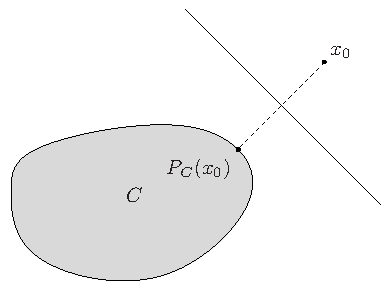
\includegraphics[width=.5\textwidth]{figures/ch08-414.pdf}
\caption*{图8.1 点 $x_0$ 及其在凸集 $C$ 上的欧氏投影 $P_C(x_0)$。位于两点中间、法向量为 $P_C(x_0)-x_0$ 的超平面，严格分离该点与集合。对一般范数，这一性质不成立，见习题8.4。}
\end{figure}
先将问题(8.2)写为
\[\begin{array}{ll}\text{最小化}&\norm y\\\text{约束为}&f_i(x)\leq0,\quad i=1,\ldots,m,\\&Ax=b,\\&x_0-x=y,\end{array}\]
变量为 $x,y$。拉格朗日函数为
\[L(x,y,\lambda,\mu,\nu)=\norm y+\sum_{i=1}^m\lambda_i f_i(x)+\nu^\T(Ax-b)+\mu^\T(x_0-x-y),\]
对偶函数为
\[g(\lambda,\mu,\nu)=\begin{cases}
 \displaystyle\inf_x\left(\sum_{i=1}^m\lambda_i f_i(x)+\nu^\T(Ax-b)+\mu^\T(x_0-x)\right),&\norm\mu_*\leq1,\\
 -\infty,&\text{其他情况}.
\end{cases}\]
于是得到对偶问题
\[\begin{array}{ll}
 \text{最大化}&\displaystyle\mu^\T x_0+\inf_x\left(\sum_{i=1}^m\lambda_if_i(x)+\nu^\T(Ax-b)-\mu^\T x\right)\\
 \text{约束为}&\lambda\succeq0,\\&\norm\mu_*\leq1,
\end{array}\]
变量为 $\lambda,\mu,\nu$。其解释如下。设 $\lambda,\mu,\nu$ 对偶可行，且对偶目标为正，即 $\lambda\succeq0$、$\norm\mu_*\leq1$，并对所有 $x$ 有
% Source PDF page 415 (printed p. 401)
\[\mu^\T x_0-\mu^\T x+\sum_{i=1}^m\lambda_if_i(x)+\nu^\T(Ax-b)>0.\]
这蕴含对 $x\in C$ 有 $\mu^\T x_0>\mu^\T x$，所以 $\mu$ 确定一个严格分离超平面。特别地，设问题(8.2)严格可行，因而强对偶成立。若 $x_0\notin C$，最优值为正，任意对偶最优解都确定一个严格分离超平面。

这个通过对偶构造分离超平面的方法适用于任意范数。相比之下，上述简单几何构造只适用于欧氏范数。
\subsubsection*{分离点与多面体}
问题
\[\begin{array}{ll}\text{最小化}&\norm y\\\text{约束为}&Ax\preceq b,\\&x_0-x=y\end{array}\]
的对偶为
\[\begin{array}{ll}\text{最大化}&\mu^\T x_0-b^\T\lambda\\\text{约束为}&A^\T\lambda=\mu,\\&\norm\mu_*\leq1,\\&\lambda\succeq0,\end{array}\]
可以进一步简化为
\[\begin{array}{ll}\text{最大化}&(Ax_0-b)^\T\lambda\\\text{约束为}&\norm{A^\T\lambda}_*\leq1,\\&\lambda\succeq0.\end{array}\]
容易验证，若对偶目标为正，$A^\T\lambda$ 就是某个分离超平面的法向量：若 $Ax\preceq b$，则
\[(A^\T\lambda)^\T x=\lambda^\T(Ax)\leq\lambda^\T b<\lambda^\T Ax_0,\]
所以 $\mu=A^\T\lambda$ 确定一个分离超平面。
\subsection{用示性函数与支撑函数表示投影和分离}
8.1.1节和8.1.2节的思路，可以用集合 $C$ 的示性函数 $I_C$ 与支撑函数 $S_C$ 紧凑地表达，其中
\[S_C(x)=\sup_{y\in C}x^\T y,\qquad
 I_C(x)=\begin{cases}0,&x\in C,\\+\infty,&x\notin C.\end{cases}\]
将 $x_0$ 投影到闭凸集 $C$ 上的问题，可紧凑地写为
\[\begin{array}{ll}\text{最小化}&\norm{x-x_0}\\\text{约束为}&I_C(x)\leq0,\end{array}\]
% Source PDF page 416 (printed p. 402)
或者等价地写为
\[\begin{array}{ll}\text{最小化}&\norm y\\\text{约束为}&I_C(x)\leq0,\\&x_0-x=y,\end{array}\]
变量为 $x,y$。其对偶函数为
\[
\begin{aligned}
 g(z,\lambda)&=\inf_{x,y}\bigl(\norm y+\lambda I_C(x)+z^\T(x_0-x-y)\bigr)\\
 &=\begin{cases}
 z^\T x_0+\inf_x(-z^\T x+I_C(x)),&\norm z_*\leq1,\ \lambda\geq0,\\
 -\infty,&\text{其他情况}
 \end{cases}\\
 &=\begin{cases}z^\T x_0-S_C(z),&\norm z_*\leq1,\ \lambda\geq0,\\-\infty,&\text{其他情况}.
 \end{cases}
\end{aligned}
\]
由此得到对偶问题
\[\begin{array}{ll}\text{最大化}&z^\T x_0-S_C(z)\\\text{约束为}&\norm z_*\leq1.\end{array}\]
若 $z$ 对偶最优且目标为正，则对所有 $x\in C$ 有 $z^\T x_0>z^\T x$，即 $z$ 确定一个分离超平面。
\section{集合之间的距离}
两个集合 $C,D$ 在范数 $\norm{\cdot}$ 下的距离定义为
\[\dist(C,D)=\inf\{\norm{x-y}\mid x\in C,\ y\in D\}.\]
若 $\dist(C,D)>0$，则 $C,D$ 不相交。若 $\dist(C,D)=0$ 且定义中的下确界能够取到，则二者相交。例如，集合都闭、其中一个有界时，下确界可取到。

集合之间的距离可用点到集合的距离表示：
\[\dist(C,D)=\dist(0,D-C),\]
因此可以应用上一节的结论。不过，本节专门针对集合间距离的问题导出结果，以便利用 $C-D$ 的结构，并使解释更直观。
\subsection{计算凸集之间的距离}
设 $C,D$ 分别由两组凸不等式描述：
\[C=\{x\mid f_i(x)\leq0,\ i=1,\ldots,m\},\qquad
 D=\{x\mid g_i(x)\leq0,\ i=1,\ldots,p\}.\]
% Source PDF page 417 (printed p. 403)
也可以加入线性等式，这里为简便而省去。求解凸优化问题
\begin{equation}
\begin{array}{ll}\text{最小化}&\norm{x-y}\\\text{约束为}&f_i(x)\leq0,\quad i=1,\ldots,m,\\&g_i(y)\leq0,\quad i=1,\ldots,p
\end{array}\tag{8.3}
\end{equation}
即可得到 $\dist(C,D)$。
\begin{figure}[htbp]\centering
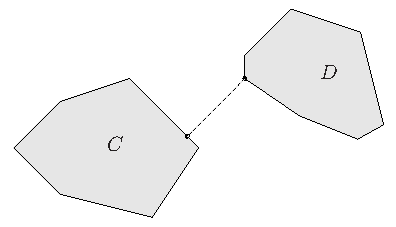
\includegraphics[width=.48\textwidth]{figures/ch08-417.pdf}
\caption*{图8.2 多面体 $C,D$ 之间的欧氏距离。虚线连接分别属于 $C,D$、欧氏距离最近的两个点。这两点可通过求解 QP 找到。}
\end{figure}
\subsubsection*{多面体之间的欧氏距离}
设多面体 $C,D$ 分别由线性不等式组 $A_1x\preceq b_1$、$A_2x\preceq b_2$ 描述。二者之间的距离，是分别属于 $C,D$ 的最近一对点的距离，见图8.2。这个距离是下列问题的最优值：
\begin{equation}\begin{array}{ll}\text{最小化}&\norm{x-y}_2\\\text{约束为}&A_1x\preceq b_1,\\&A_2y\preceq b_2.\end{array}\tag{8.4}\end{equation}
把目标平方，可以得到等价的 QP。
\subsection{分离凸集}
寻找两个凸集之间距离的问题(8.3)，其对偶通过集合之间的分离超平面具有有趣的几何解释。先将问题写成如下等价形式：
\begin{equation}\begin{array}{ll}\text{最小化}&\norm w\\\text{约束为}&f_i(x)\leq0,\quad i=1,\ldots,m,\\&g_i(y)\leq0,\quad i=1,\ldots,p,\\&x-y=w.\end{array}\tag{8.5}\end{equation}
对偶函数为
\[
 g(\lambda,z,\mu)=\inf_{x,y,w}\left(\norm w+\sum_{i=1}^m\lambda_if_i(x)
 +\sum_{i=1}^p\mu_ig_i(y)+z^\T(x-y-w)\right)
\]
% Source PDF page 418 (printed p. 404)
\[=\begin{cases}
 \displaystyle\inf_x\left(\sum_{i=1}^m\lambda_if_i(x)+z^\T x\right)
 +\inf_y\left(\sum_{i=1}^p\mu_ig_i(y)-z^\T y\right),&\norm z_*\leq1,\\
 -\infty,&\text{其他情况}.
\end{cases}\]
由此得到对偶问题
\begin{equation}\begin{array}{ll}
\text{最大化}&\displaystyle\inf_x\left(\sum_{i=1}^m\lambda_if_i(x)+z^\T x\right)
+\inf_y\left(\sum_{i=1}^p\mu_ig_i(y)-z^\T y\right)\\
\text{约束为}&\norm z_*\leq1,\\&\lambda\succeq0,\quad\mu\succeq0.
\end{array}\tag{8.6}\end{equation}
其几何解释如下。若 $\lambda,\mu$ 对偶可行且目标为正，则对所有 $x,y$ 有
\[\sum_{i=1}^m\lambda_if_i(x)+z^\T x+\sum_{i=1}^p\mu_ig_i(y)-z^\T y>0.\]
特别地，对 $x\in C$、$y\in D$，有 $z^\T x-z^\T y>0$，因此 $z$ 确定一个严格分离 $C,D$ 的超平面。

因此，若问题(8.5)与(8.6)之间强对偶成立，例如问题(8.5)严格可行，就有如下结论：若两个集合之间距离为正，就能用超平面将它们严格分离。
\subsubsection*{分离多面体}
对由线性不等式 $A_1x\preceq b_1$、$A_2x\preceq b_2$ 定义的集合应用这些对偶结果，得到对偶问题
\[\begin{array}{ll}
\text{最大化}&-b_1^\T\lambda-b_2^\T\mu\\
\text{约束为}&A_1^\T\lambda+z=0,\\&A_2^\T\mu-z=0,\\&\norm z_*\leq1,\\&\lambda\succeq0,\quad\mu\succeq0.
\end{array}\]
若 $\lambda,\mu,z$ 对偶可行，则对所有 $x\in C$、$y\in D$，
\[z^\T x=-\lambda^\T A_1x\geq-\lambda^\T b_1,\qquad
 z^\T y=\mu^\T A_2x\leq\mu^\T b_2,\]
若对偶目标为正，则
\[z^\T x-z^\T y\geq-\lambda^\T b_1-\mu^\T b_2>0,\]
即 $z$ 确定一个分离超平面。
\subsection{用示性函数与支撑函数表示距离和分离}
8.2.1节和8.2.2节的思路，可以用示性函数与支撑函数紧凑地表达。求两个凸集之间距离的问题可以写为
\[\begin{array}{ll}\text{最小化}&\norm{x-y}\\\text{约束为}&I_C(x)\leq0,\\&I_D(y)\leq0,\end{array}\]
% Source PDF page 419 (printed p. 405)
等价于
\[\begin{array}{ll}\text{最小化}&\norm w\\\text{约束为}&I_C(x)\leq0,\\&I_D(y)\leq0,\\&x-y=w.\end{array}\]
其对偶问题为
\[\begin{array}{ll}\text{最大化}&-S_C(-z)-S_D(z)\\\text{约束为}&\norm z_*\leq1.\end{array}\]
若 $z$ 对偶可行且目标为正，则 $S_D(z)<-S_C(-z)$，即
\[\sup_{x\in D}z^\T x<\inf_{x\in C}z^\T x.\]
也就是说，$z$ 确定一个严格分离 $C,D$ 的超平面。
\section{欧氏距离与角度问题}
设 $a_1,\ldots,a_n$ 是 $\R^n$ 中一组向量，暂且假设欧氏长度已知：
\[l_1=\norm{a_1}_2,\qquad\ldots,\qquad l_n=\norm{a_n}_2.\]
称这组向量为一个构形；若它们线性无关，则称为一组基。本节考虑涉及构形各种几何性质的优化问题，例如向量对之间的欧氏距离、夹角，以及刻画基的条件状况的各种几何指标。
\subsection{Gram 矩阵与可实现性}
长度、距离和角度都可以用向量 $a_1,\ldots,a_n$ 的 Gram 矩阵表示：
\[G=A^\T A,\qquad A=\begin{bmatrix}a_1&\cdots&a_n\end{bmatrix},\]
所以 $G_{ij}=a_i^\T a_j$。$G$ 的对角元为
\[G_{ii}=l_i^2,\qquad i=1,\ldots,n,\]
暂且假设它们已知且固定。$a_i$ 与 $a_j$ 之间的距离 $d_{ij}$ 为
\[\begin{aligned}
 d_{ij}&=\norm{a_i-a_j}_2\\
 &=(l_i^2+l_j^2-2a_i^\T a_j)^{1/2}\\
 &=(l_i^2+l_j^2-2G_{ij})^{1/2}.
\end{aligned}\]
% Source PDF page 420 (printed p. 406)
反过来，可以用 $d_{ij}$ 表示 $G_{ij}$：
\[G_{ij}=\frac{l_i^2+l_j^2-d_{ij}^2}2.\]
为后面引用，注意它是 $d_{ij}^2$ 的仿射函数。

非零向量 $a_i,a_j$ 之间的相关系数 $\rho_{ij}$ 为
\[\rho_{ij}=\frac{a_i^\T a_j}{\norm{a_i}_2\norm{a_j}_2}=\frac{G_{ij}}{l_il_j},\]
所以 $G_{ij}=l_il_j\rho_{ij}$ 是 $\rho_{ij}$ 的线性函数。非零向量 $a_i,a_j$ 之间的角度 $\theta_{ij}$ 为
\[\theta_{ij}=\cos^{-1}\rho_{ij}=\cos^{-1}(G_{ij}/(l_il_j)),\]
其中取 $\cos^{-1}\rho\in[0,\pi]$。因此 $G_{ij}=l_il_j\cos\theta_{ij}$。

长度、距离和角度在正交变换下保持不变：若 $Q\in\R^{n\times n}$ 正交，则向量组 $Qa_i,\ldots,Qa_n$ 具有相同的 Gram 矩阵，因而具有相同的长度、距离和角度。
\subsubsection*{可实现性}
Gram 矩阵 $G=A^\T A$ 当然对称且半正定。逆命题是线性代数的基本结论：矩阵 $G\in\mathbb S^n$ 是某组向量 $a_1,\ldots,a_n$ 的 Gram 矩阵，当且仅当 $G\succeq0$。当 $G\succeq0$ 时，求一个满足 $A^\T A=G$ 的矩阵 $A$，就能构造 Gram 矩阵为 $G$ 的构形。一个解是对称平方根 $A=G^{1/2}$。当 $G\succ0$ 时，可以通过 Cholesky 分解找到解：若 $LL^\T=G$，可取 $A=L^\T$。此外，给定任意一个解 $A$ 后，通过正交变换就能构造指定 Gram 矩阵 $G$ 的全部构形：若 $\widetilde A^\T\widetilde A=G$ 是任意解，则对某个正交矩阵 $Q$ 有 $\widetilde A=QA$。

因此，一组长度、距离和角度（或相关系数）可以实现，即来自某个构形，当且仅当相关 Gram 矩阵 $G$ 半正定，且对角元为 $l_1^2,\ldots,l_n^2$。

利用这一事实，可以把几个几何问题表示为凸优化问题，优化变量为 $G\in\mathbb S^n$。可实现性要求约束 $G\succeq0$ 以及 $G_{ii}=l_i^2$，$i=1,\ldots,n$。下面列出其他一些凸约束和目标。
\subsubsection*{角度与距离约束}
用线性等式约束 $G_{ij}=l_il_j\cos\alpha$，可以把角度固定为指定值 $\theta_{ij}=\alpha$。更一般地，用约束
\[l_il_j\cos\alpha\geq G_{ij}\geq l_il_j\cos\beta\]
可以规定角度的上下界 $\alpha\leq\theta_{ij}\leq\beta$，这是一对关于 $G$ 的线性不等式。这里使用了 $\cos^{-1}$ 单调递减。通过最小化或最大化 $G_{ij}$，也可以最大化或最小化某个角度 $\theta_{ij}$，同样利用了 $\cos^{-1}$ 的单调性。
% Source PDF page 421 (printed p. 407)
类似地也可以约束距离。要求 $d_{ij}$ 落在一个区间内，可用
\[\begin{aligned}
 d_{\min}\leq d_{ij}\leq d_{\max}
 &\Longleftrightarrow d_{\min}^2\leq d_{ij}^2\leq d_{\max}^2\\
 &\Longleftrightarrow d_{\min}^2\leq l_i^2+l_j^2-2G_{ij}\leq d_{\max}^2,
\end{aligned}\]
这是一对关于 $G$ 的线性不等式。通过最小化或最大化距离的平方，即 $G$ 的仿射函数，可以最小化或最大化距离本身。

例如，给定某些角度和某些距离的范围，即可能值的区间。通过求解两个 SDP，就能在所有构形上，找到另一个角度或另一个距离的最小、最大可能值。对最优 Gram 矩阵分解，可以重建对应的两个极端构形。
\subsubsection*{奇异值与条件数约束}
$A$ 的奇异值 $\sigma_1\geq\cdots\geq\sigma_n$ 是 $G$ 的特征值 $\lambda_1\geq\cdots\geq\lambda_n$ 的平方根。因此，$\sigma_1^2$ 是 $G$ 的凸函数，$\sigma_n^2$ 是 $G$ 的凹函数。于是，可以给 $A$ 的最大奇异值规定上界，或者将它最小化；可以给最小奇异值规定下界，或者将它最大化。$A$ 的条件数 $\sigma_1/\sigma_n$ 是 $G$ 的拟凸函数，因此可以通过拟凸优化，在满足其他几何约束的所有构形中，限制其最大允许值或将它最小化。

粗略地说，能够作为 $G$ 的凸约束施加的条件，是要求 $a_1,\ldots,a_n$ 构成条件良好的基的那些条件。
\subsubsection*{对偶基}
当 $G\succ0$ 时，$a_1,\ldots,a_n$ 构成 $\R^n$ 的一组基。对应的对偶基为 $b_1,\ldots,b_n$，满足
\[b_i^\T a_j=\begin{cases}1,&i=j,\\0,&i\ne j.\end{cases}\]
对偶基向量 $b_1,\ldots,b_n$ 就是矩阵 $A^{-1}$ 的各行。因此，对偶基的 Gram 矩阵为 $G^{-1}$。

可以把对偶基的几种几何条件写成关于 $G$ 的凸约束。对偶基向量长度的平方
\[\norm{b_i}_2^2=e_i^\T G^{-1}e_i\]
是 $G$ 的凸函数，因此可被最小化。$G^{-1}$ 的迹也是 $G$ 的凸函数，给出对偶基各向量长度平方之和，也是衡量基条件好坏的另一指标。
\subsubsection*{椭球与单纯形的体积}
椭球 $\{Au\mid\norm u_2\leq1\}$ 的体积也能衡量基的条件好坏，它为
\[\gamma(\det(A^\T A))^{1/2}=\gamma(\det G)^{1/2},\]
% Source PDF page 422 (printed p. 408)
其中 $\gamma$ 为 $\R^n$ 中单位球的体积。因此，对数体积为 $\log\gamma+\tfrac12\log\det G$，是 $G$ 的凹函数。于是，在凸的构形集合上最大化映像椭球的体积，可通过最大化 $\log\det G$ 完成。

对 $\R^n$ 中任意集合，结论相同：在 $A$ 下的像的体积，等于原体积乘以 $(\det G)^{1/2}$。例如，单位单纯形 $\conv\{0,e_1,\ldots,e_n\}$ 在 $A$ 下的像，是单纯形 $\conv\{0,a_1,\ldots,a_n\}$。其体积为 $\gamma(\det G)^{1/2}$，其中 $\gamma$ 为 $\R^n$ 中单位单纯形的体积。最大化 $\log\det G$，就能最大化这个单纯形的体积。
\subsection{只涉及角度的问题}
若只关心向量之间的角度或相关系数，不指定向量长度或彼此距离，直觉上只需假设各向量 $a_i$ 的长度 $l_i=1$。这很容易验证：Gram 矩阵具有形式 $G=\diag(l)C\diag(l)$，其中 $l$ 是长度向量，$C$ 为相关矩阵，即 $C_{ij}=\cos\theta_{ij}$。因此，若对某组正长度有 $G\succeq0$，则对任意一组正长度都有 $G\succeq0$；特别地，这当且仅当 $C\succeq0$，也就是假设所有长度均为一的情形。因此，一组角度 $\theta_{ij}\in[0,\pi]$、$i,j=1,\ldots,n$ 可实现，当且仅当 $C\succeq0$，这是关于相关系数的线性矩阵不等式。

例如，给定某些角度的上下界，等价于给某些相关系数规定上下界。通过求解两个 SDP，就能在全部构形中找到另一个角度的最小、最大可能值。
\begin{origexample}{8.3}
\textbf{相关系数的界。}考虑 $\R^4$ 中的例子，给定
\begin{equation}\begin{aligned}
 0.6\leq\rho_{12}\leq0.9,\qquad&0.8\leq\rho_{13}\leq0.9,\\
 0.5\leq\rho_{24}\leq0.7,\qquad&-0.8\leq\rho_{34}\leq-0.4.
\end{aligned}\tag{8.7}\end{equation}
为求 $\rho_{14}$ 的最小、最大可能值，求解两个 SDP：
\[\begin{array}{ll}
 \text{最小化／最大化}&\rho_{14}\\
 \text{约束为}&\text{式(8.7)},\\
 &\begin{bmatrix}1&\rho_{12}&\rho_{13}&\rho_{14}\\
 \rho_{12}&1&\rho_{23}&\rho_{24}\\
 \rho_{13}&\rho_{23}&1&\rho_{34}\\
 \rho_{14}&\rho_{24}&\rho_{34}&1\end{bmatrix}\succeq0,
\end{array}\]
变量为 $\rho_{12},\rho_{13},\rho_{14},\rho_{23},\rho_{24},\rho_{34}$。最小值、最大值取两位有效数字，分别为 $-0.39$ 和 $0.23$，对应的相关矩阵为
\[
 \begin{bmatrix}1.00&0.60&0.87&-0.39\\0.60&1.00&0.33&0.50\\0.87&0.33&1.00&-0.55\\-0.39&0.50&-0.55&1.00\end{bmatrix},\qquad
 \begin{bmatrix}1.00&0.71&0.80&0.23\\0.71&1.00&0.31&0.59\\0.80&0.31&1.00&-0.40\\0.23&0.59&-0.40&1.00\end{bmatrix}.
\]
\end{origexample}
% Source PDF page 423 (printed p. 409)
\subsection{欧氏距离问题}
在欧氏距离问题中，只关心向量之间的距离 $d_{ij}$，不关心向量的长度及其夹角。这些距离当然在正交变换下不变，而且在平移下也不变：对任意 $b\in\R^n$，构形 $\widetilde a_1=a_1+b,\ldots,\widetilde a_n=a_n+b$ 具有与原构形相同的距离。特别地，取
\[b=-\frac1n\sum_{i=1}^n a_i=-\frac1n A\one,\]
则 $\widetilde a_i$ 既保留原构形的距离，又满足 $\sum_{i=1}^n\widetilde a_i=0$。因此，在欧氏距离问题中，可以不失一般性地假设 $a_1,\ldots,a_n$ 的平均值为零，即 $A\one=0$。

求解欧氏距离问题时，可以把向量长度作为优化问题中的自由变量，这些长度本身不能出现在该类问题的目标或约束中。这里利用了如下事实：存在距离为 $d_{ij}\geq0$ 的构形，当且仅当存在长度 $l_1,\ldots,l_n$ 使 $G\succeq0$，其中 $G_{ij}=(l_i^2+l_j^2-d_{ij}^2)/2$。

定义 $z\in\R^n$、$z_i=l_i^2$，以及 $D\in\mathbb S^n$、$D_{ij}=d_{ij}^2$，当然 $D_{ii}=0$。存在某组长度使 $G\succeq0$ 的条件可写为
\begin{equation}
 G=(z\one^\T+\one z^\T-D)/2\succeq0\quad\text{对某个 }z\succeq0,\tag{8.8}
\end{equation}
这是关于 $D,z$ 的 LMI。元素非负、对角元为零且满足式(8.8)的矩阵 $D\in\mathbb S^n$，称为欧氏距离矩阵。矩阵是欧氏距离矩阵，当且仅当其元素是某个构形中向量之间欧氏距离的平方。给定欧氏距离矩阵 $D$ 及对应的长度平方向量 $z$，可用上述方法重建具有指定两两距离的一个或全部构形。

事实上，条件(8.8)等价于更简单的条件：$D$ 在 $\one^\perp$ 上半负定，即
\[\begin{aligned}
 (8.8)&\Longleftrightarrow u^\T Du\leq0\text{ 对所有满足 }\one^\T u=0\text{ 的 }u\\
 &\Longleftrightarrow(I-\tfrac1n\one\one^\T)D(I-\tfrac1n\one\one^\T)\preceq0.
\end{aligned}\]
这个简单矩阵不等式，连同 $D_{ij}\geq0$、$D_{ii}=0$，就是欧氏距离矩阵的经典刻画。为说明等价性，回顾可假设 $A\one=0$，从而 $\one^\T G\one=\one^\T A^\T A\one=0$。因此，$G\succeq0$ 当且仅当 $G$ 在 $\one^\perp$ 上半正定，即
\[\begin{aligned}
0&\preceq(I-\tfrac1n\one\one^\T)G(I-\tfrac1n\one\one^\T)\\
 &=\tfrac12(I-\tfrac1n\one\one^\T)(z\one^\T+\one z^\T-D)(I-\tfrac1n\one\one^\T)\\
 &=-\tfrac12(I-\tfrac1n\one\one^\T)D(I-\tfrac1n\one\one^\T),
\end{aligned}\]
即所需的简化条件。
% Source PDF page 424 (printed p. 410)
总之，矩阵 $D\in\mathbb S^n$ 是欧氏距离矩阵，即给出 $\R^n$ 中一组 $n$ 个向量之间的距离平方，当且仅当
\[D_{ii}=0,\quad i=1,\ldots,n,\qquad D_{ij}\geq0,\quad i,j=1,\ldots,n,\]
\[(I-\tfrac1n\one\one^\T)D(I-\tfrac1n\one\one^\T)\preceq0,\]
这是一组关于 $D$ 的线性等式、线性不等式以及矩阵不等式。因此，凡是关于距离平方凸的欧氏距离问题，都能表示为以 $D\in\mathbb S^n$ 为变量的凸问题。
\section{极值体积椭球}
设 $C\subseteq\R^n$ 有界且内部非空。本节考虑寻找位于 $C$ 内部的最大体积椭球，以及覆盖 $C$ 的最小体积椭球。这两个问题都能写成凸规划，但只有特殊情况下可有效求解。
\subsection{Löwner--John 椭球}
包含集合 $C$ 的最小体积椭球，称为 $C$ 的 Löwner--John 椭球，记为 $\mathcal E_{\mathrm{lj}}$。为刻画它，采用如下方式参数化一般椭球较为方便：
\begin{equation}\mathcal E=\{v\mid\norm{Av+b}_2\leq1\},\tag{8.9}\end{equation}
即欧氏单位球在仿射映射下的逆像。可以不失一般性地假设 $A\in\mathbb S_{++}^n$，此时 $\mathcal E$ 的体积正比于 $\det A^{-1}$。计算包含 $C$ 的最小体积椭球的问题可写为
\begin{equation}\begin{array}{ll}\text{最小化}&\log\det A^{-1}\\\text{约束为}&\sup_{v\in C}\norm{Av+b}_2\leq1,\end{array}\tag{8.10}\end{equation}
变量为 $A\in\mathbb S^n$、$b\in\R^n$，另有隐式约束 $A\succ0$。目标与约束函数关于 $A,b$ 均凸，所以问题(8.10)凸。但计算约束函数涉及求解凸函数最大化问题，只有某些特殊情况下可有效求解。
\subsubsection*{覆盖有限集的最小体积椭球}
考虑包含有限集 $C=\{x_1,\ldots,x_m\}\subseteq\R^n$ 的最小体积椭球。椭球覆盖 $C$ 当且仅当覆盖其凸包，所以覆盖 $C$ 的最小体积椭球，与包含多面体 $\conv\{x_1,\ldots,x_m\}$ 的最小体积椭球相同。
% Source PDF page 425 (printed p. 411)
应用式(8.10)，可写为
\begin{equation}\begin{array}{ll}\text{最小化}&\log\det A^{-1}\\\text{约束为}&\norm{Ax_i+b}_2\leq1,\quad i=1,\ldots,m,\end{array}\tag{8.11}\end{equation}
变量为 $A\in\mathbb S^n$、$b\in\R^n$，并有隐式约束 $A\succ0$。范数约束 $\norm{Ax_i+b}_2\leq1$ 关于 $A,b$ 是凸不等式。也可将其替换为平方形式 $\norm{Ax_i+b}_2^2\leq1$，这是关于 $A,b$ 的凸二次不等式。
\subsubsection*{覆盖椭球之并的最小体积椭球}
对于一些由二次不等式定义的集合 $C$，也能高效计算最小体积覆盖椭球。特别地，可以计算椭球的并集或和集的 Löwner--John 椭球。

例如，考虑寻找包含椭球 $\mathcal E_1,\ldots,\mathcal E_m$，从而包含它们并集的凸包，的最小体积椭球 $\mathcal E_{\mathrm{lj}}$。用凸二次不等式描述各椭球：
\[\mathcal E_i=\{x\mid x^\T A_ix+2b_i^\T x+c_i\leq0\},\qquad i=1,\ldots,m,\]
其中 $A_i\in\mathbb S_{++}^n$。将 $\mathcal E_{\mathrm{lj}}$ 参数化为
\[\begin{aligned}
 \mathcal E_{\mathrm{lj}}&=\{x\mid\norm{Ax+b}_2\leq1\}\\
 &=\{x\mid x^\T A^\T Ax+2(A^\T b)^\T x+b^\T b-1\leq0\},
\end{aligned}\]
其中 $A\in\mathbb S^n$、$b\in\R^n$。利用B.2节的结论，$\mathcal E_i\subseteq\mathcal E_{\mathrm{lj}}$ 当且仅当存在 $\tau\geq0$ 使
\[\begin{bmatrix}A^2-\tau A_i&Ab-\tau b_i\\(Ab-\tau b_i)^\T&b^\T b-1-\tau c_i\end{bmatrix}\preceq0.\]
$\mathcal E_{\mathrm{lj}}$ 的体积正比于 $\det A^{-1}$，因此求解
\[\begin{array}{ll}
\text{最小化}&\log\det A^{-1}\\
\text{约束为}&\tau_1\geq0,\ldots,\tau_m\geq0,\\
 &\begin{bmatrix}A^2-\tau_i A_i&Ab-\tau_i b_i\\(Ab-\tau_i b_i)^\T&b^\T b-1-\tau_i c_i\end{bmatrix}\preceq0,\quad i=1,\ldots,m,
\end{array}\]
可得包含全部椭球的最小体积椭球。或者，将变量 $b$ 替换为 $\widetilde b=Ab$，得到
\[\begin{array}{ll}
\text{最小化}&\log\det A^{-1}\\
\text{约束为}&\tau_1\geq0,\ldots,\tau_m\geq0,\\
 &\begin{bmatrix}
 A^2-\tau_i A_i&\widetilde b-\tau_i b_i&0\\
 (\widetilde b-\tau_i b_i)^\T&-1-\tau_i c_i&\widetilde b^\T\\
 0&\widetilde b&-A^2
 \end{bmatrix}\preceq0,\quad i=1,\ldots,m.
\end{array}\]
它关于变量 $A^2\in\mathbb S^n$、$\widetilde b$、$\tau_1,\ldots,\tau_m$ 凸。
% Source PDF page 426 (printed p. 412)
\begin{figure}[htbp]\centering
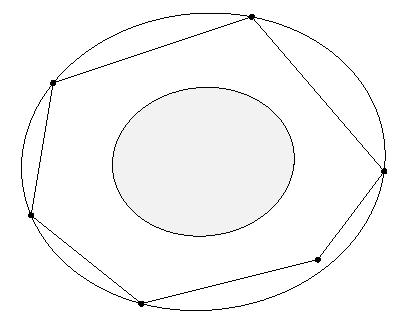
\includegraphics[width=.5\textwidth]{figures/ch08-426.pdf}
\caption*{图8.3 外侧椭圆是 Löwner--John 椭球的边界，即包围点 $x_1,\ldots,x_6$（图中的圆点），从而包围多面体 $P=\conv\{x_1,\ldots,x_6\}$ 的最小体积椭球。较小的椭圆是该椭球围绕中心缩小 $n=2$ 倍后的边界。缩小后的椭球保证位于 $P$ 内。}
\end{figure}
\subsubsection*{Löwner--John 椭球近似的效率}
设 $\mathcal E_{\mathrm{lj}}$ 为有界且内部非空的凸集 $C\subseteq\R^n$ 的 Löwner--John 椭球，中心为 $x_0$。若将该椭球围绕中心缩小 $n$ 倍，则所得椭球位于 $C$ 内：
\[x_0+\tfrac1n(\mathcal E_{\mathrm{lj}}-x_0)\subseteq C\subseteq\mathcal E_{\mathrm{lj}}.\]
换句话说，Löwner--John 椭球能够近似任意凸集，其因子只依赖于维数 $n$。图8.3给出一个简单例子。

若不对 $C$ 作额外假设，因子 $1/n$ 无法改进。例如，$\R^n$ 中任意单纯形的 Löwner--John 椭球都必须缩小 $n$ 倍才能放入其中，见习题8.13。

下面对特殊情况 $C=\conv\{x_1,\ldots,x_m\}$ 证明这一效率结论。将式(8.11)中的范数约束平方，引入 $\widetilde A=A^2$ 和 $\widetilde b=Ab$，得到
\begin{equation}\begin{array}{ll}
\text{最小化}&\log\det\widetilde A^{-1}\\
\text{约束为}&x_i^\T\widetilde A x_i-2\widetilde b^\T x_i+\widetilde b^\T\widetilde A^{-1}\widetilde b\leq1,\quad i=1,\ldots,m.
\end{array}\tag{8.12}\end{equation}
其 KKT 条件为
\[\begin{gathered}
 \sum_{i=1}^m\lambda_i(x_ix_i^\T-\widetilde A^{-1}\widetilde b\widetilde b^\T\widetilde A^{-1})=\widetilde A^{-1},\qquad
 \sum_{i=1}^m\lambda_i(x_i-\widetilde A^{-1}\widetilde b)=0,\\
 \lambda_i\geq0,\quad
 x_i^\T\widetilde A x_i-2\widetilde b^\T x_i+\widetilde b^\T\widetilde A^{-1}\widetilde b\leq1,\quad i=1,\ldots,m,\\
 \lambda_i(1-x_i^\T\widetilde A x_i+2\widetilde b^\T x_i-\widetilde b^\T\widetilde A^{-1}\widetilde b)=0,\quad i=1,\ldots,m.
\end{gathered}\]
通过适当的仿射坐标变换，可以假设 $\widetilde A=I$、$\widetilde b=0$，即最小体积椭球是以原点为中心的单位球。
% Source PDF page 427 (printed p. 413)
KKT 条件于是简化为
\[\sum_{i=1}^m\lambda_i x_ix_i^\T=I,\qquad
 \sum_{i=1}^m\lambda_i x_i=0,\qquad
 \lambda_i(1-x_i^\T x_i)=0,\quad i=1,\ldots,m,\]
再加上可行性条件 $\norm{x_i}_2\leq1$、$\lambda_i\geq0$。对第一个等式两边取迹并利用互补松弛，还得到 $\sum_{i=1}^m\lambda_i=n$。

在新坐标中，缩小后的椭球是以原点为中心、半径 $1/n$ 的球。需要证明
\[\norm x_2\leq1/n\ \Longrightarrow\ x\in C=\conv\{x_1,\ldots,x_m\}.\]
设 $\norm x_2\leq1/n$。由 KKT 条件可知
\begin{equation}
 x=\sum_{i=1}^m\lambda_i(x^\T x_i)x_i
 =\sum_{i=1}^m\lambda_i(x^\T x_i+1/n)x_i
 =\sum_{i=1}^m\mu_ix_i,\tag{8.13}
\end{equation}
其中 $\mu_i=\lambda_i(x^\T x_i+1/n)$。由 Cauchy--Schwarz 不等式，
\[\mu_i=\lambda_i(x^\T x_i+1/n)\geq\lambda_i(-\norm x_2\norm{x_i}_2+1/n)
 \geq\lambda_i(-1/n+1/n)=0.\]
此外，
\[\sum_{i=1}^m\mu_i=\sum_{i=1}^m\lambda_i(x^\T x_i+1/n)=\sum_{i=1}^m\lambda_i/n=1.\]
结合式(8.13)，说明 $x$ 是 $x_1,\ldots,x_m$ 的凸组合，从而 $x\in C$。
\subsubsection*{对称集的 Löwner--John 椭球近似效率}
若集合 $C$ 关于某点 $x_0$ 对称，则因子 $1/n$ 可以改进为 $1/\sqrt n$：
\[x_0+\tfrac1{\sqrt n}(\mathcal E_{\mathrm{lj}}-x_0)\subseteq C\subseteq\mathcal E_{\mathrm{lj}}.\]
因子 $1/\sqrt n$ 同样是紧的。立方体
\[C=\{x\in\R^n\mid-\one\preceq x\preceq\one\}\]
的 Löwner--John 椭球是半径 $\sqrt n$ 的球。将其缩小 $\sqrt n$ 倍，得到包含在 $C$ 中、并在 $x=\pm e_i$ 处与边界相切的球。
\subsubsection*{用二次范数近似范数}
设 $\norm{\cdot}$ 是 $\R^n$ 上任意范数，$C=\{x\mid\norm x\leq1\}$ 是其单位球。设 $\mathcal E_{\mathrm{lj}}=\{x\mid x^\T Ax\leq1\}$、$A\in\mathbb S_{++}^n$ 是 $C$ 的 Löwner--John 椭球。由于 $C$ 关于原点对称，上述结果说明 $(1/\sqrt n)\mathcal E_{\mathrm{lj}}\subseteq C\subseteq\mathcal E_{\mathrm{lj}}$。

用 $\norm{\cdot}_{\mathrm{lj}}$ 表示二次范数
\[\norm z_{\mathrm{lj}}=(z^\T Az)^{1/2},\]
% Source PDF page 428 (printed p. 414)
其单位球为 $\mathcal E_{\mathrm{lj}}$。包含关系 $(1/\sqrt n)\mathcal E_{\mathrm{lj}}\subseteq C\subseteq\mathcal E_{\mathrm{lj}}$ 等价于对所有 $z\in\R^n$ 的不等式
\[\norm z_{\mathrm{lj}}\leq\norm z\leq\sqrt n\norm z_{\mathrm{lj}}.\]
换句话说，二次范数 $\norm{\cdot}_{\mathrm{lj}}$ 在 $\sqrt n$ 因子内近似范数 $\norm{\cdot}$。特别地，$\R^n$ 上任意范数都可以由二次范数在 $\sqrt n$ 因子内近似。
\subsection{最大体积内接椭球}
现在考虑寻找位于凸集 $C$ 内的最大体积椭球，其中假设 $C$ 有界且内部非空。为建立模型，将椭球参数化为单位球在仿射变换下的像，即
\[\mathcal E=\{Bu+d\mid\norm u_2\leq1\}.\]
仍可以假设 $B\in\mathbb S_{++}^n$，体积因而正比于 $\det B$。求解凸优化问题
\begin{equation}\begin{array}{ll}
\text{最大化}&\log\det B\\
\text{约束为}&\sup_{\norm u_2\leq1} I_C(Bu+d)\leq0
\end{array}\tag{8.14}\end{equation}
即可求得 $C$ 内的最大体积椭球，变量为 $B\in\mathbb S^n$、$d\in\R^n$，隐式约束为 $B\succ0$。
\subsubsection*{多面体中的最大体积椭球}
考虑 $C$ 是由线性不等式组描述的多面体：
\[C=\{x\mid a_i^\T x\leq b_i,\ i=1,\ldots,m\}.\]
为应用式(8.14)，先把约束改写为更方便的形式：
\[\begin{aligned}
 \sup_{\norm u_2\leq1}I_C(Bu+d)\leq0
 &\Longleftrightarrow\sup_{\norm u_2\leq1}a_i^\T(Bu+d)\leq b_i,\quad i=1,\ldots,m\\
 &\Longleftrightarrow\norm{Ba_i}_2+a_i^\T d\leq b_i,\quad i=1,\ldots,m.
\end{aligned}\]
于是将式(8.14)表示为关于变量 $B,d$ 的凸优化问题：
\begin{equation}\begin{array}{ll}\text{最小化}&\log\det B^{-1}\\\text{约束为}&\norm{Ba_i}_2+a_i^\T d\leq b_i,\quad i=1,\ldots,m.\end{array}\tag{8.15}\end{equation}
\subsubsection*{椭球交集中的最大体积椭球}
也可以寻找位于 $m$ 个椭球 $\mathcal E_1,\ldots,\mathcal E_m$ 交集内的最大体积椭球 $\mathcal E$。用 $\mathcal E=\{Bu+d\mid\norm u_2\leq1\}$、$B\in\mathbb S_{++}^n$ 描述它；其他椭球用凸二次不等式描述：
\[\mathcal E_i=\{x\mid x^\T A_ix+2b_i^\T x+c_i\leq0\},\quad i=1,\ldots,m,\]
% Source PDF page 429 (printed p. 415)
其中 $A_i\in\mathbb S_{++}^n$。先求出 $\mathcal E\subseteq\mathcal E_i$ 的条件。这当且仅当
\[\begin{aligned}
 &\sup_{\norm u_2\leq1}\bigl((d+Bu)^\T A_i(d+Bu)+2b_i^\T(d+Bu)+c_i\bigr)\\
 &\quad=d^\T A_id+2b_i^\T d+c_i
 +\sup_{\norm u_2\leq1}\bigl(u^\T BA_iBu+2(A_id+b_i)^\T Bu\bigr)\leq0.
\end{aligned}\]
根据B.1节，
\[\sup_{\norm u_2\leq1}\bigl(u^\T BA_iBu+2(A_id+b_i)^\T Bu\bigr)
 \leq-(d^\T A_id+2b_i^\T d+c_i)\]
当且仅当存在 $\lambda_i\geq0$ 使
\[\begin{bmatrix}
 -\lambda_i-d^\T A_id-2b_i^\T d-c_i&(A_id+b_i)^\T B\\
 B(A_id+b_i)&\lambda_i I-BA_iB
\end{bmatrix}\succeq0.\]
因此，求解
\[\begin{array}{ll}
\text{最小化}&\log\det B^{-1}\\
\text{约束为}&\begin{bmatrix}
 -\lambda_i-d^\T A_id-2b_i^\T d-c_i&(A_id+b_i)^\T B\\
 B(A_id+b_i)&\lambda_i I-BA_iB
\end{bmatrix}\succeq0,\quad i=1,\ldots,m,
\end{array}\]
可求得包含在 $\mathcal E_1,\ldots,\mathcal E_m$ 中的最大体积椭球，变量为 $B\in\mathbb S^n$、$d\in\R^n$、$\lambda\in\R^m$。等价地，求解
\[\begin{array}{ll}
\text{最小化}&\log\det B^{-1}\\
\text{约束为}&\begin{bmatrix}
 -\lambda_i-c_i+b_i^\T A_i^{-1}b_i&0&(d+A_i^{-1}b_i)^\T\\
 0&\lambda_i I&B\\
 d+A_i^{-1}b_i&B&A_i^{-1}
 \end{bmatrix}\succeq0,\quad i=1,\ldots,m.
\end{array}\]
\subsubsection*{椭球内近似的效率}
最大体积内接椭球也有与 Löwner--John 椭球类似的近似效率结论。若 $C\subseteq\R^n$ 凸、有界且内部非空，则将最大体积内接椭球围绕中心扩大 $n$ 倍，就能覆盖 $C$。若集合关于某点对称，因子 $n$ 可改进为 $\sqrt n$。图8.4给出一个例子。
\subsection{极值体积椭球的仿射不变性}
Löwner--John 椭球和最大体积内接椭球都具有仿射不变性。若 $\mathcal E_{\mathrm{lj}}$ 是 $C$ 的 Löwner--John 椭球，$T\in\R^{n\times n}$ 非奇异，则 $TC$ 的 Löwner--John 椭球是 $T\mathcal E_{\mathrm{lj}}$。最大体积内接椭球也有类似结论。

为证明这一结论，设 $\mathcal E$ 是任意覆盖 $C$ 的椭球，则 $T\mathcal E$ 覆盖 $TC$。反过来也成立：覆盖 $TC$ 的每个椭球都具有 $T\mathcal E$ 的形式，其中 $\mathcal E$ 覆盖 $C$。
% Source PDF page 430 (printed p. 416)
\begin{figure}[htbp]\centering
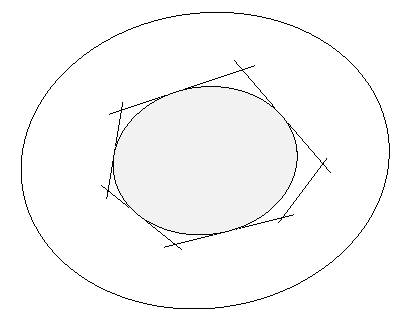
\includegraphics[width=.5\textwidth]{figures/ch08-430.pdf}
\caption*{图8.4 内接于多面体 $P$ 的最大体积椭球，以阴影表示。外侧椭圆是内椭球围绕中心扩大 $n=2$ 倍后的边界。扩大的椭球保证覆盖 $P$。}
\end{figure}
换句话说，关系 $\widetilde{\mathcal E}=T\mathcal E$ 建立了覆盖 $TC$ 的椭球与覆盖 $C$ 的椭球之间的一一对应。此外，对应椭球的体积之比都是 $|\det T|$，因此特别地，若 $\mathcal E$ 在覆盖 $C$ 的椭球中体积最小，则 $T\mathcal E$ 在覆盖 $TC$ 的椭球中体积最小。
\section{求中心}
\subsection{Chebyshev 中心}
设 $C\subseteq\R^n$ 有界、内部非空，$x\in C$。点 $x\in C$ 的深度定义为
\[\operatorname{depth}(x,C)=\dist(x,\R^n\setminus C),\]
即到 $C$ 外部最近点的距离。深度给出了以 $x$ 为中心、位于 $C$ 内的最大球的半径。集合 $C$ 的 Chebyshev 中心定义为 $C$ 中任意深度最大的点：
\[x_{\mathrm{cheb}}(C)=\argmax\operatorname{depth}(x,C)
 =\argmax\dist(x,\R^n\setminus C).\]
Chebyshev 中心是 $C$ 内离外部最远的点，也是位于 $C$ 内的最大球的中心。图8.5给出 $C$ 为多面体、范数为欧氏范数的例子。
% Source PDF page 431 (printed p. 417)
\begin{figure}[htbp]\centering
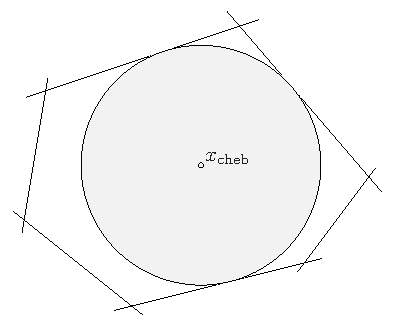
\includegraphics[width=.5\textwidth]{figures/ch08-431.pdf}
\caption*{图8.5 欧氏范数下多面体 $C$ 的 Chebyshev 中心。中心 $x_{\mathrm{cheb}}$ 是 $C$ 内最深的点，即离 $C$ 的外部或补集最远的点。它也是位于 $C$ 内的最大欧氏球（浅色阴影）的中心。}
\end{figure}
\subsubsection*{凸集的 Chebyshev 中心}
当集合 $C$ 凸时，深度是 $x\in C$ 的凹函数，因此计算 Chebyshev 中心是凸优化问题，见习题8.5。具体地，设 $C\subseteq\R^n$ 由一组凸不等式定义：
\[C=\{x\mid f_1(x)\leq0,\ldots,f_m(x)\leq0\}.\]
可通过求解问题
\begin{equation}\begin{array}{ll}\text{最大化}&R\\\text{约束为}&g_i(x,R)\leq0,\quad i=1,\ldots,m,\end{array}\tag{8.16}\end{equation}
找到 Chebyshev 中心，其中
\[g_i(x,R)=\sup_{\norm u\leq1}f_i(x+Ru).\]
问题(8.16)是凸优化问题，因为每个 $g_i$ 都是一族关于 $x,R$ 的凸函数的逐点最大值，因此凸。但计算 $g_i$ 需要以数值或解析方式求解凸函数最大化问题，这可能非常困难。实际中，只有 $g_i$ 容易计算时，才能求出 Chebyshev 中心。
\subsubsection*{多面体的 Chebyshev 中心}
设 $C$ 由线性不等式组 $a_i^\T x\leq b_i$、$i=1,\ldots,m$ 定义。当 $R\geq0$ 时有
\[g_i(x,R)=\sup_{\norm u\leq1}\bigl(a_i^\T(x+Ru)-b_i\bigr)
 =a_i^\T x+R\norm{a_i}_*-b_i.\]
% Source PDF page 432 (printed p. 418)
因此，求解 LP
\[\begin{array}{ll}\text{最大化}&R\\\text{约束为}&a_i^\T x+R\norm{a_i}_*\leq b_i,\quad i=1,\ldots,m,\\&R\geq0,\end{array}\]
即可得到 Chebyshev 中心，变量为 $x,R$。
\subsubsection*{椭球交集的欧氏 Chebyshev 中心}
设 $C$ 为 $m$ 个椭球的交，由二次不等式定义：
\[C=\{x\mid x^\T A_ix+2b_i^\T x+c_i\leq0,\ i=1,\ldots,m\},\]
其中 $A_i\in\mathbb S_{++}^n$。有
\[\begin{aligned}
 g_i(x,R)&=\sup_{\norm u_2\leq1}\bigl((x+Ru)^\T A_i(x+Ru)+2b_i^\T(x+Ru)+c_i\bigr)\\
 &=x^\T A_ix+2b_i^\T x+c_i
 +\sup_{\norm u_2\leq1}\bigl(R^2u^\T A_iu+2R(A_ix+b_i)^\T u\bigr).
\end{aligned}\]
由B.1节，$g_i(x,R)\leq0$ 当且仅当存在 $\lambda_i$ 使矩阵不等式
\begin{equation}\begin{bmatrix}
 -x^\T A_ix_i-2b_i^\T x-c_i-\lambda_i&R(A_ix+b_i)^\T\\
 R(A_ix+b_i)&\lambda_i I-R^2A_i
\end{bmatrix}\succeq0\tag{8.17}\end{equation}
成立。利用这一结论，可将 Chebyshev 中心问题写成
\[\begin{array}{ll}
\text{最大化}&R\\
\text{约束为}&\begin{bmatrix}
 -\lambda_i-c_i+b_i^\T A_i^{-1}b_i&0&(x+A_i^{-1}b_i)^\T\\
 0&\lambda_i I&RI\\
 x+A_i^{-1}b_i&RI&A_i^{-1}
 \end{bmatrix}\succeq0,\quad i=1,\ldots,m,
\end{array}\]
这是以 $R,\lambda,x$ 为变量的 SDP。LMI 约束中 $A_i^{-1}$ 的 Schur 补，恰为式(8.17)的左端。
\subsection{最大体积椭球中心}
集合 $C\subseteq\R^n$ 的 Chebyshev 中心 $x_{\mathrm{cheb}}$，是位于 $C$ 内的最大球的中心。推广这一想法，将 $C$ 的最大体积椭球中心 $x_{\mathrm{mve}}$ 定义为位于 $C$ 内的最大体积椭球的中心。图8.6给出 $C$ 为多面体的例子。

当 $C$ 由一组线性不等式定义时，求解问题(8.15)即可得到最大体积椭球中心，变量 $d\in\R^n$ 的最优值就是 $x_{\mathrm{mve}}$。由于 $C$ 内的最大体积椭球具有仿射不变性，最大体积椭球中心也具有仿射不变性。
% Source PDF page 433 (printed p. 419)
\begin{figure}[htbp]\centering
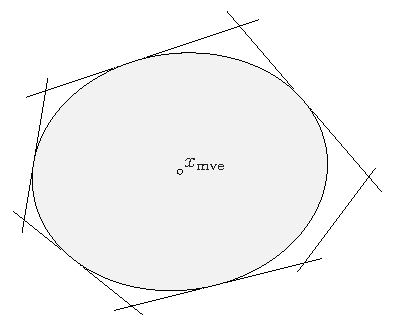
\includegraphics[width=.5\textwidth]{figures/ch08-433.pdf}
\caption*{图8.6 浅色阴影椭球为集合 $C$ 内的最大体积椭球，这里的 $C$ 与图8.5为同一个多面体。它的中心 $x_{\mathrm{mve}}$ 就是 $C$ 的最大体积椭球中心。}
\end{figure}
\subsection{不等式组的解析中心}
凸不等式与线性等式组
\[f_i(x)\leq0,\quad i=1,\ldots,m,\qquad Fx=g\]
的解析中心 $x_{\mathrm{ac}}$，定义为以下凸问题的一个最优点：
\begin{equation}\begin{array}{ll}\text{最小化}&-\sum_{i=1}^m\log(-f_i(x))\\\text{约束为}&Fx=g,\end{array}\tag{8.18}\end{equation}
变量为 $x\in\R^n$，隐式约束为 $f_i(x)<0$、$i=1,\ldots,m$。式(8.18)中的目标称为与该不等式组关联的对数障碍。这里假设对数障碍的定义域与等式定义的仿射集相交，即严格不等式组
\[f_i(x)<0,\quad i=1,\ldots,m,\qquad Fx=g\]
可行。若可行集
\[C=\{x\mid f_i(x)<0,\ i=1,\ldots,m,\ Fx=g\}\]
有界，则对数障碍在可行集上有下界。

当 $x$ 严格可行，即 $Fx=g$ 且各 $f_i(x)<0$ 时，可将 $-f_i(x)$ 理解为第 $i$ 条不等式的裕量或松弛量。解析中心 $x_{\mathrm{ac}}$ 是满足等式约束 $Fx=g$ 及隐式约束 $f_i(x)<0$，并使这些松弛量或裕量的乘积（或几何平均）最大的点。

解析中心不是由不等式与等式描述的集合 $C$ 的函数：两组不等式与等式可以定义同一个集合，却具有不同解析中心。尽管如此，人们仍常非正式地使用“集合 $C$ 的解析中心”，来指代定义该集合的某组等式与不等式的解析中心。
% Source PDF page 434 (printed p. 420)
不过，解析中心不依赖于仿射坐标变换。它也在不等式函数的正数缩放、以及等式约束的任意重新参数化下保持不变。换句话说，若 $\widetilde F,\widetilde g$ 使 $\widetilde Fx=\widetilde g$ 当且仅当 $Fx=g$，且 $\alpha_1,\ldots,\alpha_m>0$，则
\[\alpha_i f_i(x)\leq0,\quad i=1,\ldots,m,\qquad\widetilde Fx=\widetilde g\]
的解析中心，与
\[f_i(x)\leq0,\quad i=1,\ldots,m,\qquad Fx=g\]
的解析中心相同，见习题8.17。
\subsubsection*{线性不等式组的解析中心}
线性不等式组
\[a_i^\T x\leq b_i,\qquad i=1,\ldots,m\]
的解析中心是无约束最小化问题
\begin{equation}\text{最小化}\quad-\sum_{i=1}^m\log(b_i-a_i^\T x)\tag{8.19}\end{equation}
的解，隐式约束为 $b_i-a_i^\T x>0$、$i=1,\ldots,m$。若线性不等式定义的多面体有界，则对数障碍有下界且严格凸，因此解析中心唯一，见习题4.2。

线性不等式组的解析中心有一个几何解释。由于解析中心不依赖于约束函数的正数缩放，可以不失一般性地假设 $\norm{a_i}_2=1$。此时，松弛量 $b_i-a_i^\T x$ 是到超平面 $H_i=\{x\mid a_i^\T x=b_i\}$ 的距离。因此，解析中心 $x_{\mathrm{ac}}$ 使到各定义超平面距离的乘积最大。
\subsubsection*{由线性不等式解析中心得到的内、外椭球}
线性不等式组的解析中心，通过对数障碍函数
\[-\sum_{i=1}^m\log(b_i-a_i^\T x)\]
在解析中心处的 Hessian，隐式确定一个内接椭球和一个覆盖椭球。该 Hessian 为
\[H=\sum_{i=1}^m d_i^2a_ia_i^\T,\qquad
 d_i=\frac1{b_i-a_i^\T x_{\mathrm{ac}}},\quad i=1,\ldots,m.\]
有 $\mathcal E_{\mathrm{inner}}\subseteq P\subseteq\mathcal E_{\mathrm{outer}}$，其中
\[\begin{aligned}
P&=\{x\mid a_i^\T x\leq b_i,\ i=1,\ldots,m\},\\
\mathcal E_{\mathrm{inner}}&=\{x\mid(x-x_{\mathrm{ac}})^\T H(x-x_{\mathrm{ac}})\leq1\},\\
\mathcal E_{\mathrm{outer}}&=\{x\mid x-x_{\mathrm{ac}})^\T H(x-x_{\mathrm{ac}})\leq m(m-1)\}.
\end{aligned}\]
% Source PDF page 435 (printed p. 421)
\begin{figure}[htbp]\centering
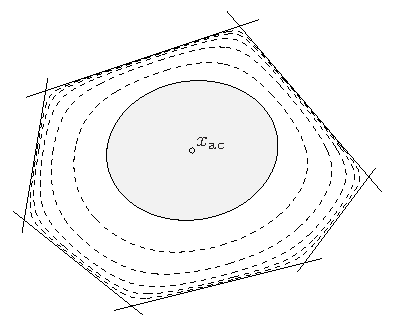
\includegraphics[width=.5\textwidth]{figures/ch08-435.pdf}
\caption*{图8.7 虚线为定义图8.5中多面体 $C$ 的不等式组所对应对数障碍函数的五条等高线。标为 $x_{\mathrm{ac}}$ 的对数障碍最小点，是不等式组的解析中心。内椭球 $\mathcal E_{\mathrm{inner}}=\{x\mid(x-x_{\mathrm{ac}})H(x-x_{\mathrm{ac}})\leq1\}$ 以阴影表示，其中 $H$ 为对数障碍在 $x_{\mathrm{ac}}$ 处的 Hessian。}
\end{figure}
这个结论比最大体积内接椭球的结论弱，后者扩大 $n$ 倍就覆盖多面体。对数障碍 Hessian 所定义的内、外椭球，其缩放因子为 $(m(m-1))^{1/2}$，总不小于 $n$。

为证明 $\mathcal E_{\mathrm{inner}}\subseteq P$，设 $x\in\mathcal E_{\mathrm{inner}}$，即
\[(x-x_{\mathrm{ac}})^\T H(x-x_{\mathrm{ac}})
 =\sum_{i=1}^m(d_i a_i^\T(x-x_{\mathrm{ac}}))^2\leq1.\]
这说明
\[a_i^\T(x-x_{\mathrm{ac}})\leq1/d_i=b_i-a_i^\T x_{\mathrm{ac}},\qquad i=1,\ldots,m,\]
所以对所有 $i$ 有 $a_i^\T x\leq b_i$。这里并未使用 $x_{\mathrm{ac}}$ 是解析中心，因此把 $x_{\mathrm{ac}}$ 换成任意严格可行点，结论仍成立。

为证明 $P\subseteq\mathcal E_{\mathrm{outer}}$，需要用到 $x_{\mathrm{ac}}$ 为解析中心这一事实，因此对数障碍梯度为零：
\[\sum_{i=1}^m d_ia_i=0.\]
现在假设 $x\in P$，则
\[\begin{aligned}
 (x-x_{\mathrm{ac}})^\T H(x-x_{\mathrm{ac}})
 &=\sum_{i=1}^m(d_i a_i^\T(x-x_{\mathrm{ac}}))^2\\
% Source PDF page 436 (printed p. 422)
 &=\sum_{i=1}^m d_i^2(1/d_i-a_i^\T(x-x_{\mathrm{ac}}))^2-m\\
 &=\sum_{i=1}^m d_i^2(b_i-a_i^\T x)^2-m\\
 &\leq\left(\sum_{i=1}^m d_i(b_i-a_i^\T x)\right)^2-m\\
 &=\left(\sum_{i=1}^m d_i(b_i-a_i^\T x_{\mathrm{ac}})
       +\sum_{i=1}^m d_i a_i^\T(x_{\mathrm{ac}}-x)\right)^2-m\\
 &=m^2-m,
\end{aligned}\]
表明 $x\in\mathcal E_{\mathrm{outer}}$。第二个等式来自 $\sum_{i=1}^m d_ia_i=0$；不等式来自对 $y\succeq0$ 成立的 $\sum_{i=1}^m y_i^2\leq(\sum_{i=1}^m y_i)^2$；最后一个等式使用了 $\sum_{i=1}^m d_ia_i=0$ 和 $d_i$ 的定义。
\subsubsection*{线性矩阵不等式的解析中心}
若在锥 $K$ 上定义对数，解析中心的定义就能推广到由相对于 $K$ 的广义不等式描述的集合。例如，线性矩阵不等式
\[x_1A_1+x_2A_2+\cdots+x_nA_n\preceq B\]
的解析中心，定义为
\[\text{最小化}\quad-\log\det(B-x_1A_1-\cdots-x_nA_n)\]
的解。
\section{分类}
在模式识别和分类问题中，给定 $\R^n$ 中两组点 $\{x_1,\ldots,x_N\}$、$\{y_1,\ldots,y_M\}$，希望在指定函数族中找到 $f:\R^n\to\R$，使它在第一组点上为正，在第二组点上为负，即
\[f(x_i)>0,\quad i=1,\ldots,N,\qquad f(y_i)<0,\quad i=1,\ldots,M.\]
若这些不等式成立，就说 $f$ 或其零水平集 $\{x\mid f(x)=0\}$ 分离、分类或判别了两组点。有时也考虑弱分离，即上述不等式取非严格形式。
% Source PDF page 437 (printed p. 423)
\begin{figure}[htbp]\centering
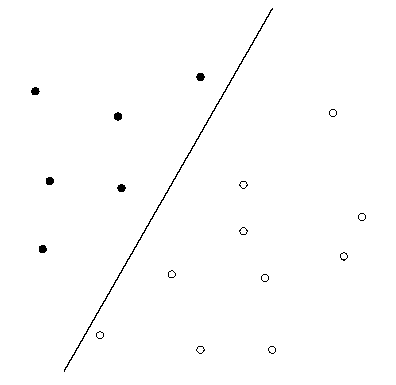
\includegraphics[width=.48\textwidth]{figures/ch08-437.pdf}
\caption*{图8.8 点 $x_1,\ldots,x_N$ 以空心圆表示，点 $y_1,\ldots,y_M$ 以实心圆表示。仿射函数 $f$ 对这两组点进行分类，它的零水平集是一条分离二者的直线。}
\end{figure}
\subsection{线性判别}
线性判别要寻找对点分类的仿射函数 $f(x)=a^\T x-b$，即
\begin{equation}a^\T x_i-b>0,\quad i=1,\ldots,N,\qquad
 a^\T y_i-b<0,\quad i=1,\ldots,M.\tag{8.20}\end{equation}
几何上，就是寻找分离两组点的超平面。由于严格不等式(8.20)关于 $a,b$ 齐次，它们可行当且仅当关于变量 $a,b$ 的非严格线性不等式组
\begin{equation}a^\T x_i-b\geq1,\quad i=1,\ldots,N,\qquad
 a^\T y_i-b\leq-1,\quad i=1,\ldots,M\tag{8.21}\end{equation}
可行。图8.8给出两组点与线性判别函数的一个简单例子。
\subsubsection*{线性判别的择一定理}
严格不等式组(8.20)的强择一条件，是存在 $\lambda,\widetilde\lambda$ 使
\begin{equation}\begin{gathered}
 \lambda\succeq0,\quad\widetilde\lambda\succeq0,\quad(\lambda,\widetilde\lambda)\ne0,\\
 \sum_{i=1}^N\lambda_ix_i=\sum_{i=1}^M\widetilde\lambda_i y_i,\qquad
 \one^\T\lambda=\one^\T\widetilde\lambda.
\end{gathered}\tag{8.22}\end{equation}
见5.8.3节。利用第三个和最后一个条件，可将择一条件写为
\[\lambda\succeq0,\quad\one^\T\lambda=1,\quad
 \widetilde\lambda\succeq0,\quad\one^\T\widetilde\lambda=1,\quad
 \sum_{i=1}^N\lambda_ix_i=\sum_{i=1}^M\widetilde\lambda_i y_i.\]
% Source PDF page 438 (printed p. 424)
这里除以正数 $\one^\T\lambda$，并沿用原符号表示归一化后的 $\lambda,\widetilde\lambda$。这些条件的几何含义很简单：存在一个点同时属于 $\{x_1,\ldots,x_N\}$ 与 $\{y_1,\ldots,y_M\}$ 的凸包。换句话说，两组点能够线性判别，即用仿射函数判别，当且仅当其凸包不相交。前面已多次遇到这一结论。
\subsubsection*{稳健线性判别}
存在仿射分类函数 $f(x)=a^\T x-b$，等价于定义该函数的变量 $a,b$ 满足一组线性不等式。若两组点可线性判别，则判别它们的仿射函数构成一个多面体，可以选择其中使某种稳健性指标最优的函数。例如，可以寻找在 $x_i$ 处的正值与 $y_i$ 处的负值之间具有最大可能间隔的函数。为此必须归一化 $a,b$，否则将二者乘以正常数就能使函数值间隔任意大。这导出问题
\begin{equation}\begin{array}{ll}
\text{最大化}&t\\
\text{约束为}&a^\T x_i-b\geq t,\quad i=1,\ldots,N,\\
&a^\T y_i-b\leq-t,\quad i=1,\ldots,M,\\
&\norm a_2\leq1,
\end{array}\tag{8.23}\end{equation}
变量为 $a,b,t$。这个凸问题具有线性目标、线性不等式以及一个二次不等式；其最优值 $t^\star$ 为正，当且仅当两组点可线性判别。此时，$\norm a_2\leq1$ 在最优点总取等号，即 $\norm{a^\star}_2=1$，见习题8.23。

稳健线性判别问题(8.23)有简单的几何解释。若 $\norm a_2=1$，任意最优点都满足这一点，则 $a^\T x_i-b$ 是 $x_i$ 到分离超平面 $H=\{z\mid a^\T z=b\}$ 的欧氏距离。同样，$b-a^\T y_i$ 为 $y_i$ 到该超平面的距离。因此，问题(8.23)寻找既分离两组点、又与它们距离最大的超平面。也就是说，它寻找能分离两组点的最厚平板。

如图8.9所示，最优值 $t^\star$，即平板厚度的一半，事实上等于两组点凸包之间距离的一半。这可从问题(8.23)的对偶清楚地看出。对最小化 $-t$ 的问题，拉格朗日函数为
\[-t+\sum_{i=1}^N u_i(t+b-a^\T x_i)
 +\sum_{i=1}^M v_i(t-b+a^\T y_i)+\lambda(\norm a_2-1).\]
对 $b,t$ 最小化，得到条件 $\one^\T u=1/2$、$\one^\T v=1/2$。这些条件成立时，
\[g(u,v,\lambda)=\inf_a\left(a^\T\left(\sum_{i=1}^M v_iy_i-\sum_{i=1}^N u_ix_i\right)+\lambda\norm a_2\right)-\lambda\]
% Source PDF page 439 (printed p. 425)
\[=\begin{cases}
 -\lambda,&\left\|\sum_{i=1}^M v_iy_i-\sum_{i=1}^N u_ix_i\right\|_2\leq\lambda,\\
 -\infty,&\text{其他情况}.
\end{cases}\]
对偶问题于是可写为
\[\begin{array}{ll}
\text{最大化}&-\left\|\sum_{i=1}^M v_iy_i-\sum_{i=1}^N u_ix_i\right\|_2\\
\text{约束为}&u\succeq0,\quad\one^\T u=1/2,\\&v\succeq0,\quad\one^\T v=1/2.
\end{array}\]
可将 $2\sum_{i=1}^N u_ix_i$ 解释为 $\{x_1,\ldots,x_N\}$ 凸包中的点，$2\sum_{i=1}^M v_iy_i$ 解释为 $\{y_1,\ldots,y_M\}$ 凸包中的点。对偶目标是最小化这两点距离的一半，即寻找两个凸包距离的一半。
\begin{figure}[htbp]\centering
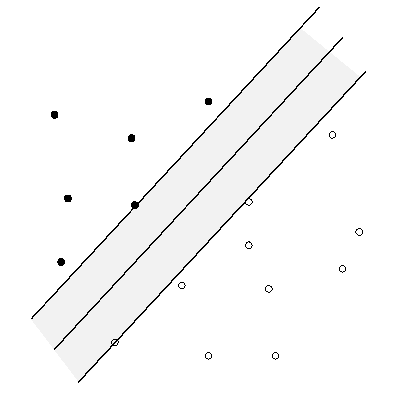
\includegraphics[width=.5\textwidth]{figures/ch08-439.pdf}
\caption*{图8.9 求解稳健线性判别问题(8.23)，得到一个仿射函数，使两组点上的函数值具有最大间隔，其中线性部分受归一化约束。几何上，这是寻找分离两组点的最厚平板。}
\end{figure}
\subsubsection*{支持向量分类器}
两组点无法线性分离时，可以寻找近似分类的仿射函数，例如使误分类点数最小的函数。遗憾的是，这一般是困难的组合优化问题。本节介绍一种基于支持向量分类器的近似线性判别启发式方法。

从可行性问题(8.21)出发，先引入非负变量 $u_1,\ldots,u_N$ 和 $v_1,\ldots,u_M$，放宽约束为
\begin{equation}a^\T x_i-b\geq1-u_i,\quad i=1,\ldots,N,\qquad
 a^\T y_i-b\leq-(1-v_i),\quad i=1,\ldots,M.\tag{8.24}\end{equation}
% Source PDF page 440 (printed p. 426)
\begin{figure}[htbp]\centering
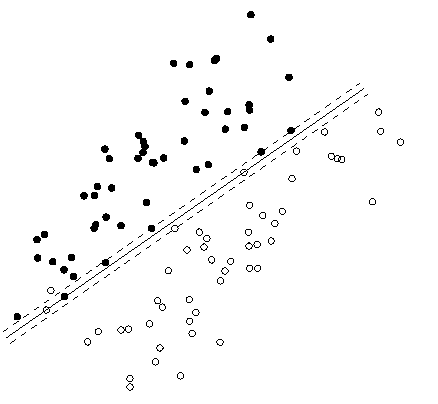
\includegraphics[width=.54\textwidth]{figures/ch08-440.pdf}
\caption*{图8.10 通过线性规划进行近似线性判别。空心圆为 $x_1,\ldots,x_{50}$，实心圆为 $y_1,\ldots,y_{50}$，两组点无法线性分离。实线分类器由 LP(8.25)求得，误分类一个点。虚线为超平面 $a^\T z-b=\pm1$。有四个点分类正确，但位于两条虚线定义的平板内。}
\end{figure}
当 $u=v=0$ 时，恢复原约束；将 $u,v$ 取得充分大，总能使这些不等式可行。可以把 $u_i$ 看作约束 $a^\T x_i-b\geq1$ 的违反程度，$v_i$ 类似。目标是找到 $a,b$ 以及稀疏非负向量 $u,v$，使不等式(8.24)成立。一种启发式做法是最小化各 $u_i,v_i$ 之和，即求解 LP
\begin{equation}\begin{array}{ll}
\text{最小化}&\one^\T u+\one^\T v\\
\text{约束为}&a^\T x_i-b\geq1-u_i,\quad i=1,\ldots,N,\\
&a^\T y_i-b\leq-(1-v_i),\quad i=1,\ldots,M,\\
&u\succeq0,\quad v\succeq0.
\end{array}\tag{8.25}\end{equation}
图8.10给出一个例子，仿射函数 $a^\T z-b$ 将100个点中的一个误分类。不过，当 $0<u_i<1$ 时，点 $x_i$ 被该仿射函数正确分类，却违反不等式 $a^\T x_i-b\geq1$，$y_i$ 的情况类似。LP(8.25)的目标可以解释为以下数量的松弛：违反 $a^\T x_i-b\geq1$ 的 $x_i$ 个数，加上违反 $a^\T y_i-b\leq-1$ 的 $y_i$ 个数。换句话说，它松弛了函数 $a^\T z-b$ 的误分类点数，加上分类正确但位于 $-1<a^\T z-b<1$ 平板内的点数。

更一般地，可以权衡误分类点数与平板 $\{z\mid-1\leq a^\T z-b\leq1\}$ 的宽度，后者为 $2/\norm a_2$。点集 $\{x_1,\ldots,x_N\}$、$\{y_1,\ldots,y_M\}$ 的标准支持向量分类器，
% Source PDF page 441 (printed p. 427)
定义为以下问题的解：
\[\begin{array}{ll}
\text{最小化}&\norm a_2+\gamma(\one^\T u+\one^\T v)\\
\text{约束为}&a^\T x_i-b\geq1-u_i,\quad i=1,\ldots,N,\\
&a^\T y_i-b\leq-(1-v_i),\quad i=1,\ldots,M,\\&u\succeq0,\quad v\succeq0.
\end{array}\]
第一项正比于平板 $-1\leq a^\T z-b\leq1$ 宽度的倒数。第二项与上面的解释相同，是误分类点数的凸松弛，其中也包括平板内的点。正参数 $\gamma$ 给出误分类点数（希望减小）相对于平板宽度（希望增大）的权重。图8.11给出一个例子。
\begin{figure}[htbp]\centering
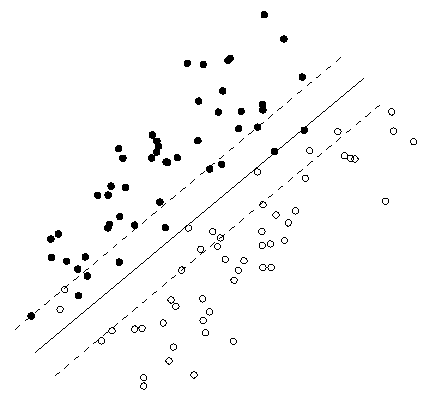
\includegraphics[width=.5\textwidth]{figures/ch08-441.pdf}
\caption*{图8.11 支持向量分类器的近似线性判别，$\gamma=0.1$。实线表示的支持向量分类器误分类三个点。有十五个点分类正确，但落在两条虚线围成的平板 $-1<a^\T z-b<1$ 内。}
\end{figure}
\subsubsection*{通过 logistic 模型进行近似线性判别}
另一种为无法线性分离的两组点寻找近似分类仿射函数的方法，是采用7.1.1节的 logistic 模型。先用 logistic 模型拟合两组点。设随机变量 $z$ 取值零或一，分布通过如下 logistic 模型依赖于确定性解释变量 $u\in\R^n$：
\begin{equation}\begin{aligned}
 \Prob(z=1)&=\frac{\exp(a^\T u-b)}{1+\exp(a^\T u-b)},\\
 \Prob(z=0)&=\frac1{1+\exp(a^\T u-b)}.
\end{aligned}\tag{8.26}\end{equation}
现在假设，给定点集 $\{x_1,\ldots,x_N\}$ 与 $\{y_1,\ldots,y_M\}$ 来自这个 logistic 模型的样本。具体地，$\{x_1,\ldots,x_N\}$ 是 $z=1$ 的 $N$ 个样本所对应的 $u$ 值，$\{y_1,\ldots,y_M\}$ 是 $z=0$ 的 $M$ 个样本所对应的 $u$ 值。
% Source PDF page 442 (printed p. 428)
这允许 $x_i=y_j$，而这种情况会使两组点无法判别。在 logistic 模型中，这只表示两个样本的解释变量相同、结果不同。

从观测样本出发，通过最大似然估计确定 $a,b$，即求解以 $a,b$ 为变量的凸优化问题
\begin{equation}\text{最小化}\quad-l(a,b),\tag{8.27}\end{equation}
其中 $l$ 为对数似然函数，
\[\begin{aligned}
 l(a,b)&=\sum_{i=1}^N(a^\T x_i-b)\\
 &\quad-\sum_{i=1}^N\log(1+\exp(a^\T x_i-b))
       -\sum_{i=1}^M\log(1+\exp(a^\T y_i-b)),
\end{aligned}\]
见7.1.1节。若两组点可线性分离，即存在 $a,b$ 使 $a^\T x_i>b$、$a^\T y_i<b$，则优化问题(8.27)向下无界。

找到 $a,b$ 的最大似然值后，可为两组点建立线性分类器 $f(x)=a^\T x-b$。假设数据点确实由参数为 $a,b$ 的 logistic 模型生成，这个分类器在所有线性分类器中具有最小误分类概率。超平面 $a^\T u=b$ 对应于 $\Prob(z=1)=1/2$ 的点，即两种结果同样可能。图8.12给出一个例子。
\paragraph{注8.1}\textbf{Bayes 解释。}设 $x,z$ 为分别取值于 $\R^n$ 与 $\{0,1\}$ 的随机变量。假设
\[\Prob(z=1)=\Prob(z=0)=1/2,\]
以 $p_0(x),p_1(x)$ 分别表示给定 $z=0$、$z=1$ 时 $x$ 的条件概率密度。假设存在 $a,b$ 使
\[\frac{p_1(x)}{p_0(x)}=e^{a^\T x-b}.\]
许多常见分布满足这一性质。例如，$p_0,p_1$ 可以是 $\R^n$ 上协方差相同、均值不同的两个正态密度，也可以是 $\R_+^n$ 上的两个指数密度。

由 Bayes 公式，
\[\Prob(z=1\mid x=u)=\frac{p_1(u)}{p_1(u)+p_0(u)},\qquad
 \Prob(z=0\mid x=u)=\frac{p_0(u)}{p_1(u)+p_0(u)},\]
从而得到
\[\begin{aligned}
 \Prob(z=1\mid x=u)&=\frac{\exp(a^\T u-b)}{1+\exp(a^\T u-b)},\\
 \Prob(z=0\mid x=u)&=\frac1{1+\exp(a^\T u-b)}.
\end{aligned}\]
% Source PDF page 443 (printed p. 429)
因此，可以把 logistic 模型(8.26)解释为给定 $x=u$ 时 $z$ 的后验分布。
\begin{figure}[htbp]\centering
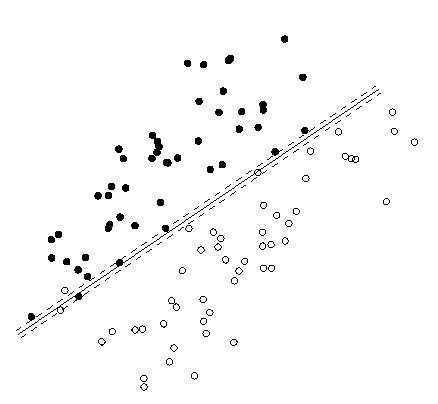
\includegraphics[width=.5\textwidth]{figures/ch08-443.pdf}
\caption*{图8.12 通过 logistic 模型进行近似线性判别。空心圆为 $x_1,\ldots,x_{50}$，实心圆为 $y_1,\ldots,y_{50}$，它们无法线性分离。最大似然 logistic 模型给出深色直线表示的超平面，仅误分类两个点。两条虚线表示 $a^\T u-b=\pm1$，按 logistic 模型，各自对应结果的概率为73\%。有三个点分类正确，但位于两条虚线之间。}
\end{figure}
\subsection{非线性判别}
同样可以在给定函数子空间中寻找非线性函数 $f$，使它在一组点上为正、另一组点上为负：
\[f(x_i)>0,\quad i=1,\ldots,N,\qquad f(y_i)<0,\quad i=1,\ldots,M.\]
只要 $f$ 对定义它的参数是线性或仿射的，这些不等式就能以与线性判别完全相同的方式求解。本节考察几个有趣的特殊情况。
\subsubsection*{二次判别}
设 $f$ 为二次函数：$f(x)=x^\T Px+q^\T x+r$。参数 $P\in\mathbb S^n$、$q\in\R^n$、$r\in\R$ 必须满足
\[x_i^\T Px_i+q^\T x_i+r>0,\quad i=1,\ldots,N,\]
\[y_i^\T Py_i+q^\T y_i+r<0,\quad i=1,\ldots,M,\]
% Source PDF page 444 (printed p. 430)
这是关于变量 $P,q,r$ 的一组严格线性不等式。如同线性判别，$f$ 关于 $P,q,r$ 齐次，因此求解非严格可行性问题
\[x_i^\T Px_i+q^\T x_i+r\geq1,\quad i=1,\ldots,N,\]
\[y_i^\T Py_i+q^\T y_i+r\leq-1,\quad i=1,\ldots,M\]
就能找到严格不等式的解。

分离曲面 $\{z\mid z^\T Pz+q^\T z+r=0\}$ 是二次曲面，两个分类区域
\[\{z\mid z^\T Pz+q^\T z+r\leq0\},\qquad
 \{z\mid z^\T Pz+q^\T z+r\geq0\}\]
由二次不等式定义。因此，求解二次判别问题，等同于判断两组点是否能被二次曲面分离。

通过增加对 $P,q,r$ 的约束，可以规定分离曲面或分类区域的形状。例如，要求 $P\prec0$，意味着分离曲面为椭球面。具体地，就是寻找包含所有 $x_1,\ldots,x_N$，而不含任何 $y_1,\ldots,y_M$ 的椭球。这个二次判别问题可以写成 SDP 可行性问题
\[\begin{array}{ll}
\text{寻找}&P,q,r\\
\text{约束为}&x_i^\T Px_i+q^\T x_i+r\geq1,\quad i=1,\ldots,N,\\
&y_i^\T Py_i+q^\T y_i+r\leq-1,\quad i=1,\ldots,M,\\&P\preceq-I,
\end{array}\]
变量为 $P\in\mathbb S^n$、$q\in\R^n$、$r\in\R$。这里利用关于 $P,q,r$ 的齐次性，将 $P\prec0$ 表示成 $P\preceq-I$。图8.13给出一个例子。
\subsubsection*{多项式判别}
考虑 $\R^n$ 上次数不超过 $d$ 的多项式集合：
\[f(x)=\sum_{i_1+\cdots+i_n\leq d}a_{i_1\cdots i_d}x_1^{i_1}\cdots x_n^{i_n}.\]
求解关于变量 $a_{i_1\cdots i_d}$ 的一组线性不等式，就能确定两组点 $\{x_1,\ldots,x_N\}$、$\{y_1,\ldots,y_M\}$ 能否由这样的多项式分离。几何上，就是检验二者能否由次数不超过 $d$ 的多项式定义的代数曲面分离。

进一步，寻找能分离两组点的最低次数 $\R^n$ 上多项式，可以通过拟凸规划求解，因为多项式次数是系数的拟凸函数。可对 $d$ 二分，每一步求解一个线性规划可行性问题。图8.14给出一个例子。
% Source PDF page 445 (printed p. 431)
\begin{figure}[htbp]\centering
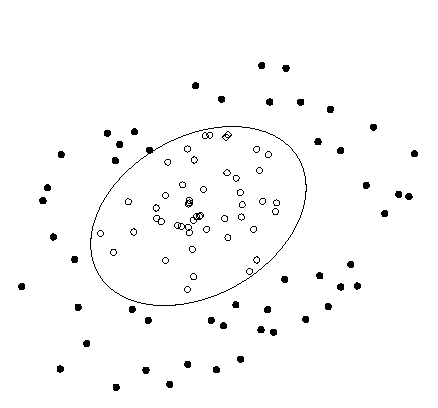
\includegraphics[width=.5\textwidth]{figures/ch08-445a.pdf}
\caption*{图8.13 二次判别，条件为 $P\prec0$。这意味着寻找包含所有 $x_i$（空心圆）且不含任何 $y_i$（实心圆）的椭球。可将其作为 SDP 可行性问题求解。}
\end{figure}
\begin{figure}[htbp]\centering
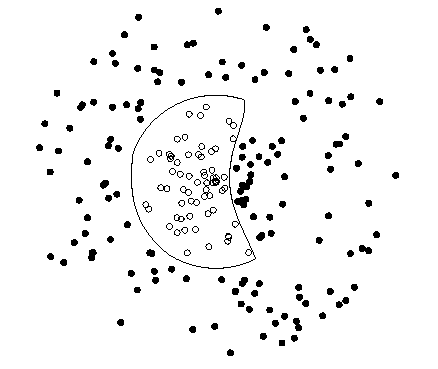
\includegraphics[width=.5\textwidth]{figures/ch08-445b.pdf}
\caption*{图8.14 $\R^2$ 中的最低次数多项式判别。本例中，不存在三次多项式能将 $x_1,\ldots,x_N$（空心圆）与 $y_1,\ldots,y_M$（实心圆）分离，但四次多项式可以，图中画出了它的零水平集。}
\end{figure}
% Source PDF page 446 (printed p. 432)
\section{布置与选址}
本节讨论下列问题的几个变体：在 $\R^2$ 或 $\R^3$ 中有 $N$ 个点，以及必须用链路相连的点对列表。部分点的位置固定；任务是确定其余点的位置，即布置其余点。目标是在满足额外位置约束的条件下，使链路总连接长度的某种度量最小。

例如，可将各点看作公司工厂或仓库的位置，链路看作运输货物的路线，目标是寻找使总运输成本最小的位置。在另一应用中，各点表示集成电路中模块或单元的位置，链路表示连接单元对的导线，目标可以是使连接所有单元的导线总长最小。

用含 $N$ 个节点的无向图描述问题，每个节点代表一个点。与每个节点关联变量 $x_i\in\R^k$，其中 $k=2$ 或 $k=3$，表示其位置。问题是最小化
\[\sum_{(i,j)\in\mathcal A}f_{ij}(x_i,x_j),\]
其中 $\mathcal A$ 是图中全部链路的集合，$f_{ij}:\R^k\times\R^k\to\R$ 为弧 $(i,j)$ 的代价函数。也可以对全部 $i,j$，或对 $i<j$ 求和，在节点 $i,j$ 不相连时令 $f_{ij}=0$。部分坐标向量 $x_i$ 已给定，优化变量为其余坐标。只要各 $f_{ij}$ 凸，这就是凸优化问题。
\subsection{线性设施选址问题}
最简单的版本中，弧 $(i,j)$ 的代价是节点 $i,j$ 之间的距离：$f_{ij}(x_i,x_j)=\norm{x_i-x_j}$，即最小化
\[\sum_{(i,j)\in\mathcal A}\norm{x_i-x_j}.\]
可以采用任意范数，最常见的是欧氏范数与 $\ell_1$ 范数。例如，在电路设计中，单元间的导线通常沿分段线性路径布设，每段为水平或竖直。这称为 Manhattan 布线，因为矩形街区城市中的街道路径也是分段线性的，每条街道沿两条正交轴之一。此时，连接单元 $i,j$ 所需导线长度为 $\norm{x_i-x_j}_1$。

还可以加入非负权重，反映不同弧上单位距离成本的差异：
% Source PDF page 447 (printed p. 433)
\[\sum_{(i,j)\in\mathcal A}w_{ij}\norm{x_i-x_j}.\]
将不相连节点对的权重设为 $w_{ij}=0$，就可更简洁地用目标
\begin{equation}\sum_{i<j}w_{ij}\norm{x_i-x_j}\tag{8.28}\end{equation}
表示这一问题。这个布置问题凸。
\begin{origexample}{8.4}
\textbf{一个自由点。}考虑只有点 $(u,v)\in\R^2$ 自由的情况，最小化它到固定点 $(u_1,v_1),\ldots,(u_K,v_K)$ 的距离之和。
\begin{itemize}
\item \textbf{$\ell_1$ 范数。}可以解析地求出使
\[\sum_{i=1}^K(|u-u_i|+|v-v_i|)\]
最小的点。任意坐标中位点均为最优点，即 $u$ 可取 $\{u_1,\ldots,u_K\}$ 的任意中位数，$v$ 可取 $\{v_1,\ldots,v_K\}$ 的任意中位数。若 $K$ 为奇数，最小点唯一；若 $K$ 为偶数，最优点可能构成一个矩形。
\item \textbf{欧氏范数。}使欧氏距离之和
\[\sum_{i=1}^K\bigl((u-u_i)^2+(v-v_i)^2\bigr)^{1/2}\]
最小的点 $(u,v)$，称为这些固定点的 Weber 点。
\end{itemize}
\end{origexample}
\subsection{布置约束}
下面列举可以加入基本布置问题、并保持凸性的一些约束。可以要求某些位置 $x_i$ 属于指定凸集，例如某条直线、区间、正方形或椭球；可以限制一个点相对于其他一个或多个点的位置，例如限制一对点之间的距离；也可以规定相对位置，例如某点必须位于另一点左侧。

一组点的包围盒是包含这些点的最小矩形。例如，通过加入约束
\[u\preceq x_i\preceq v,\quad i=1,\ldots,p,\qquad2\one^\T(v-u)\leq P_{\max},\]
可以要求点 $x_1,\ldots,x_p$ 位于周长不超过 $P_{\max}$ 的包围盒内，其中 $u,v$ 为附加变量。
% Source PDF page 448 (printed p. 434)
\subsection{非线性设施选址问题}
更一般地，可以给每条弧指定一个关于长度非线性递增的代价，即
\[\text{最小化}\quad\sum_{i<j}w_{ij}h(\norm{x_i-x_j}),\]
其中 $h$ 在 $\R_+$ 上递增且凸，$w_{ij}\geq0$。称为非线性布置或非线性设施选址问题。

一种常见情况采用欧氏范数与 $h(z)=z^2$，即最小化
\[\sum_{i<j}w_{ij}\norm{x_i-x_j}_2^2.\]
它称为二次布置问题。若仅有线性等式约束，可解析求解；若约束为线性等式与不等式，则可作为 QP 求解。
\begin{origexample}{8.5}
\textbf{一个自由点。}考虑仅有一个点 $x$ 自由，最小化到固定点 $x_1,\ldots,x_K$ 的欧氏距离平方之和：
\[\norm{x-x_1}_2^2+\norm{x-x_2}_2^2+\cdots+\norm{x-x_K}_2^2.\]
求导可知，最优 $x$ 为
\[\frac1K(x_1+x_2+\cdots+x_K),\]
即固定点的平均值。
\end{origexample}
其他一些有意义的选择包括死区宽度为 $2\gamma$ 的死区函数 $h$，定义为
\[h(z)=\begin{cases}0,&|z|\leq\gamma,\\|z-\gamma|,&|z|\geq\gamma,\end{cases}\]
以及二次—线性函数 $h$，定义为
\[h(z)=\begin{cases}z^2,&|z|\leq\gamma,\\2\gamma|z|-\gamma^2,&|z|\geq\gamma.\end{cases}\]
\begin{origexample}{8.6}
考虑 $\R^2$ 中具有6个自由点、8个固定点和27条链路的布置问题。图8.15—8.17展示分别采用准则
\[\sum_{(i,j)\in\mathcal A}\norm{x_i-x_j}_2,\qquad
 \sum_{(i,j)\in\mathcal A}\norm{x_i-x_j}_2^2,\qquad
 \sum_{(i,j)\in\mathcal A}\norm{x_i-x_j}_2^4\]
的最优解，即分别使用惩罚函数 $h(z)=z$、$h(z)=z^2$、$h(z)=z^4$。图中还给出了相应链路长度的分布。

比较结果可见，线性布置将自由点集中在小区域内，二次和四次布置则将点分散在更大区域。线性布置包含许多很短的链路和少数很长的链路：3条短于0.2，2条长于1.5。二次惩罚相对于短链路，更重地惩罚长链路；对于短于0.1的链路，惩罚几乎可忽略。
% Source PDF page 449 (printed p. 435)
\begin{figure}[htbp]\centering
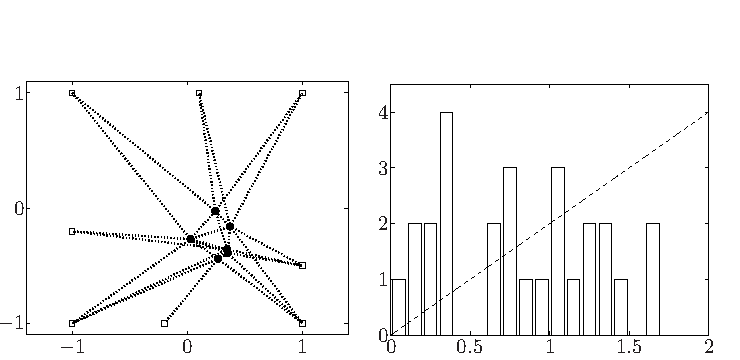
\includegraphics[width=.85\textwidth]{figures/ch08-449a.pdf}
\caption*{图8.15 线性布置。问题包含6个自由点（圆点）、8个固定点（方块）和27条链路。自由点坐标使链路欧氏长度之和最小。右图给出27条链路长度的分布。虚线是缩放后的惩罚函数 $h(z)=z$。}
\end{figure}
\begin{figure}[htbp]\centering
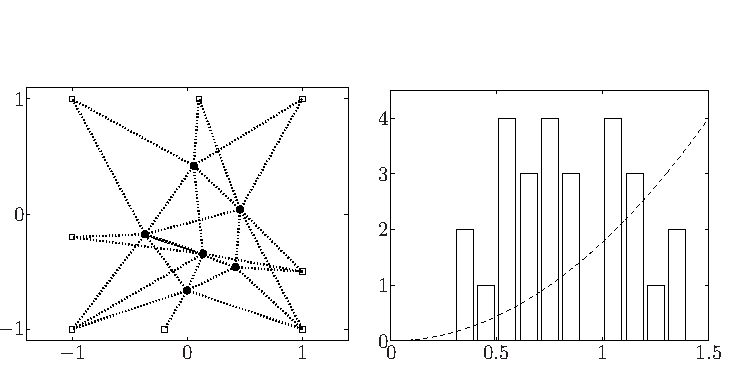
\includegraphics[width=.85\textwidth]{figures/ch08-449b.pdf}
\caption*{图8.16 二次布置。与图8.15采用相同数据，使链路欧氏长度平方和最小。虚线是缩放后的惩罚函数 $h(z)=z^2$。}
\end{figure}
% Source PDF page 450 (printed p. 436)
\begin{figure}[htbp]\centering
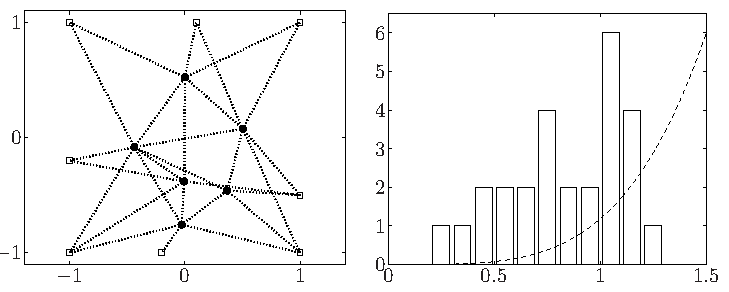
\includegraphics[width=.85\textwidth]{figures/ch08-450.pdf}
\caption*{图8.17 四次布置。使链路欧氏长度的四次方之和最小。虚线是缩放后的惩罚函数 $h(z)=z^4$。}
\end{figure}
因此，二次布置的最大长度更短，小于1.4，但短链路也更少。四次函数对长链路的惩罚更重，在更宽的区间（零至约0.4）内几乎可忽略。因此，最大长度比二次布置更短，但接近最大长度的链路也更多。
\end{origexample}
\subsection{带路径约束的选址问题}
\subsubsection*{路径约束}
沿点 $x_1,\ldots,x_N$ 的一条含 $p$ 条链路的路径，由节点序列 $i_0,\ldots,i_p\in\{1,\ldots,N\}$ 描述。路径长度为
\[\norm{x_{i_1}-x_{i_0}}+\norm{x_{i_2}-x_{i_1}}+\cdots+\norm{x_{i_p}-x_{i_{p-1}}},\]
这是 $x_1,\ldots,x_N$ 的凸函数，因此对路径长度规定上界是凸约束。有些有意义的布置问题包含路径约束，或目标基于路径长度。下面介绍一个典型例子，目标是一组路径中的最大路径长度。
\subsubsection*{极小极大延迟布置}
考虑节点为 $1,\ldots,N$ 的有向无环图，弧或链路由有序对集合 $\mathcal A$ 表示：$(i,j)\in\mathcal A$ 当且仅当有一条弧从 $i$ 指向 $j$。若没有 $\mathcal A$ 中的弧指向节点 $i$，称其为源节点；若没有弧从它离开，称其为汇节点或目的节点。关心图中从源节点开始、在汇节点结束的极大路径。

图中的弧用于表示某种流，例如货物或信息，在节点位置为 $x_1,\ldots,x_N$ 的网络中流动。流从一个源节点开始，
% Source PDF page 451 (printed p. 437)
沿路径逐个节点移动，最后到达汇节点或目的节点。用相邻节点间距离描述货物的传播时间或运输时间；一条路径的总延迟或传播时间，正比于相邻节点距离之和。

现在可以描述极小极大延迟布置问题：部分节点位置固定，其余位置自由，即为优化变量；目标是选择自由节点位置，使任意源节点至汇节点路径的最大总延迟最小。这显然是凸问题，因为目标
\begin{equation}\begin{split}
T_{\max}=\max\{&\norm{x_{i_1}-x_{i_0}}+\cdots+\norm{x_{i_p}-x_{i_{p-1}}}\mid\\
 &i_0,\ldots,i_p\text{ 为源节点至汇节点的路径}\}
\end{split}\tag{8.29}\end{equation}
是位置 $x_1,\ldots,x_N$ 的凸函数。

虽然最小化式(8.29)是凸问题，源至汇路径的数量却可能很大，随节点数或弧数指数增长。有一种有用的重新表述，可以避免枚举所有源至汇路径。

先说明如何计算最大延迟 $T_{\max}$，其效率远高于逐条计算源至汇路径的延迟再取最大值。令 $\tau_k$ 为从节点 $k$ 到某个汇节点的全部路径中最大总延迟。若 $k$ 为汇节点，显然 $\tau_k=0$。考虑节点 $k$，它的出弧通向节点 $j_1,\ldots,j_p$。从 $k$ 出发、到汇节点结束的路径，第一条弧必通向这些节点之一。若路径先到 $j_i$，再沿从那里到汇节点的最长路径，总长度为
\[\norm{x_{j_i}-x_k}+\tau_{j_i},\]
即通向 $j_i$ 的弧长，加上 $j_i$ 到汇节点的最长路径总长。因此，从 $k$ 到汇节点的路径最大延迟满足
\begin{equation}
 \tau_k=\max\{\norm{x_{j_1}-x_k}+\tau_{j_1},\ldots,\norm{x_{j_p}-x_k}+\tau_{j_p}\}.\tag{8.30}
\end{equation}
这是一个简单的动态规划论证。

等式(8.30)给出计算任意节点最大延迟的递推：从最大延迟为零的汇节点出发，利用式(8.30)反向推进，直到全部源节点。这类路径的最大延迟就是所有 $\tau_k$ 的最大值，并将在某个源节点取得。这一动态规划递推表明，无须枚举全部路径，就能递归计算任意源至汇路径上的最大延迟。所需算术运算次数约等于链路数。

下面利用基于式(8.30)的递推，建立极小极大延迟布置问题。可将问题写为
\[\begin{array}{ll}
\text{最小化}&\max\{\tau_k\mid k\text{ 为源节点}\}\\
\text{约束为}&\tau_k=0,\quad k\text{ 为汇节点},\\
&\tau_k=\max\{\norm{x_j-x_k}+\tau_j\mid\text{存在从 }k\text{ 到 }j\text{ 的弧}\},
\end{array}\]
% Source PDF page 452 (printed p. 438)
变量为 $\tau_1,\ldots,\tau_N$ 及自由位置。这个问题不凸，但将等式替换为不等式后，可得到等价的凸形式。引入新变量 $T_1,\ldots,T_N$，分别作为 $\tau_1,\ldots,\tau_N$ 的上界。所有汇节点取 $T_k=0$，用不等式
\[T_k\geq\max\{\norm{x_{j_1}-x_k}+T_{j_1},\ldots,\norm{x_{j_p}-x_k}+T_{j_p}\}\]
代替式(8.30)。若这些不等式成立，则 $T_k\geq\tau_k$。建立问题
\[\begin{array}{ll}
\text{最小化}&\max\{T_k\mid k\text{ 为源节点}\}\\
\text{约束为}&T_k=0,\quad k\text{ 为汇节点},\\
&T_k\geq\max\{\norm{x_j-x_k}+T_j\mid\text{存在从 }k\text{ 到 }j\text{ 的弧}\}.
\end{array}\]
它以 $T_1,\ldots,T_N$ 及自由位置为变量，是凸问题，并求解了极小极大延迟选址问题。
\section{平面布局}
在布置问题中，变量表示需要最优放置的若干点的坐标。平面布局问题可以看作从两个方面推广布置问题：
\begin{itemize}
\item 待放置对象是与坐标轴对齐的矩形或盒，而不是点，且不能重叠；
\item 每个矩形或盒可以在一定范围内重新配置。例如，固定各矩形的面积，但不分别固定长度与高度。
\end{itemize}
目标通常是最小化包围盒的大小，例如面积、体积或周长；包围盒是包含全部待配置、待放置盒子的最小盒。

不重叠约束使一般平面布局成为复杂的组合优化或矩形装填问题。不过，若已指定盒子的相对位置，有几类布局问题可以建立为凸优化。本节研究其中一些，主要考虑二维情况，对高维推广中不明显之处作简要说明。

有 $N$ 个单元或模块 $C_1,\ldots,C_N$，需要配置并放入宽 $W$、高 $H$、左下角在 $(0,0)$ 的矩形内。第 $i$ 个单元的几何形状和位置，由宽 $w_i$、高 $h_i$ 以及左下角坐标 $(x_i,y_i)$ 指定，见图8.18。

问题变量为 $x_i,y_i,w_i,h_i$，$i=1,\ldots,N$，以及外包矩形的宽 $W$ 和高 $H$。所有布局问题都要求各单元位于外包矩形内，即
\begin{equation}
 x_i\geq0,\quad y_i\geq0,\quad x_i+w_i\leq W,\quad y_i+h_i\leq H,\quad i=1,\ldots,N.\tag{8.31}
\end{equation}
% Source PDF page 453 (printed p. 439)
\begin{figure}[htbp]\centering
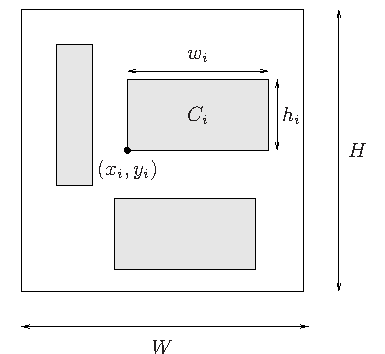
\includegraphics[width=.5\textwidth]{figures/ch08-453.pdf}
\caption*{图8.18 平面布局问题。将不重叠的矩形单元放入宽 $W$、高 $H$、左下角为 $(0,0)$ 的矩形内。第 $i$ 个单元由宽 $w_i$、高 $h_i$ 及左下角坐标 $(x_i,y_i)$ 指定。}
\end{figure}
还要求各单元除边界外不重叠：
\[\operatorname{int}(C_i\cap C_j)=\varnothing,\qquad i\ne j.\]
也可以要求单元之间有正的最小间隙。不重叠约束成立，当且仅当对 $i\ne j$，以下条件至少一个成立：$C_i$ 位于 $C_j$ 左侧、右侧、下方或上方。

这四个几何条件对应于不等式
\begin{equation}
 x_i+w_i\leq x_j,\quad\text{或 }x_j+w_j\leq x_i,\quad
 \text{或 }y_i+h_i\leq y_j,\quad\text{或 }y_j+h_j\leq y_i,\tag{8.32}
\end{equation}
对每个 $i\ne j$ 至少一条成立。这些约束具有组合性质：每一对不同单元，四个不等式中至少一个必须成立。
\subsection{相对位置约束}
相对位置约束的思路是，为每一对单元指定四种可能位置关系中的一种，即左、右、上、下。一个简单方法是在 $\{1,\ldots,N\}$ 上给出两个关系：$\mathcal L$ 表示“位于左侧”，$\mathcal B$ 表示“位于下方”。规定 $(i,j)\in\mathcal L$ 时，$C_i$ 位于 $C_j$ 左侧；$(i,j)\in\mathcal B$ 时，$C_i$ 位于 $C_j$ 下方。于是得到约束
\begin{equation}
 x_i+w_i\leq x_j\text{ 对 }(i,j)\in\mathcal L,\qquad
 y_i+h_i\leq y_j\text{ 对 }(i,j)\in\mathcal B,\tag{8.33}
\end{equation}
% Source PDF page 454 (printed p. 440)
其中 $i,j=1,\ldots,N$。为确保 $\mathcal L,\mathcal B$ 指定每对单元的相对位置，要求对每个 $i\ne j$，以下之一成立：
\[(i,j)\in\mathcal L,\qquad(j,i)\in\mathcal L,\qquad
 (i,j)\in\mathcal B,\qquad(j,i)\in\mathcal B,\]
并要求 $(i,i)\notin\mathcal L$、$(i,i)\notin\mathcal B$。不等式(8.33)是关于变量的 $N(N-1)/2$ 条线性不等式。它们蕴含不重叠不等式(8.32)，后者由 $N(N-1)/2$ 个“四条线性不等式的析取”组成。

可以假设 $\mathcal L,\mathcal B$ 反对称，即 $(i,j)\in\mathcal L\Rightarrow(j,i)\notin\mathcal L$，并且传递，即 $(i,j)\in\mathcal L$、$(j,k)\in\mathcal L\Rightarrow(i,k)\in\mathcal L$。否则相对位置约束显然不可行。传递性对应于一个直接的条件：若 $C_i$ 在 $C_j$ 左侧，而 $C_j$ 在 $C_k$ 左侧，则 $C_i$ 必在 $C_k$ 左侧。此时 $(i,k)\in\mathcal L$ 对应的不等式冗余，由另外两条蕴含。利用关系 $\mathcal L,\mathcal B$ 的传递性，可以删除冗余约束，得到紧凑的相对位置不等式组。

最小的相对位置约束集，可以方便地用两个有向无环图 $\mathcal H,\mathcal V$ 描述，分别表示水平与竖直。两个图都含 $N$ 个节点，对应布局中的 $N$ 个单元。图 $\mathcal H$ 生成关系 $\mathcal L$：$(i,j)\in\mathcal L$ 当且仅当 $\mathcal H$ 中存在从 $i$ 到 $j$ 的有向路径。类似地，$\mathcal V$ 生成 $\mathcal B$：$(i,j)\in\mathcal B$ 当且仅当 $\mathcal V$ 中存在从 $i$ 到 $j$ 的有向路径。为确保每对单元都有相对位置约束，要求在两个图之一中，存在从这对单元之一通向另一单元的有向路径。

显然，只需施加两个图中边所对应的不等式，其余都由传递性推出。于是得到
\begin{equation}
 x_i+w_i\leq x_j\text{ 对 }(i,j)\in\mathcal H,\qquad
 y_i+h_i\leq y_j\text{ 对 }(i,j)\in\mathcal V,\tag{8.34}
\end{equation}
每条边对应一条线性不等式。式(8.34)是式(8.33)的子集，并与之等价。

同样，$4N$ 条不等式(8.31)可以缩减为最小等价组。约束 $x_i\geq0$ 只需对最左侧单元施加，即在关系 $\mathcal L$ 中极小的 $i$；它们对应 $\mathcal H$ 中无入边的源节点。类似地，$x_i+w_i\leq W$ 只需对最右侧单元施加。竖直方向的外包盒不等式也可以同样精简。得到最小等价外包盒约束：
\begin{equation}\begin{aligned}
 x_i&\geq0\text{ 对 }\mathcal L\text{ 中极小的 }i,&x_i+w_i&\leq W\text{ 对 }\mathcal L\text{ 中极大的 }i,\\
 y_i&\geq0\text{ 对 }\mathcal B\text{ 中极小的 }i,&y_i+h_i&\leq H\text{ 对 }\mathcal B\text{ 中极大的 }i.
\end{aligned}\tag{8.35}\end{equation}
图8.19给出一个简单例子。其中，$\mathcal L$ 中极小、即最左侧的单元为 $C_1,C_2,C_4$，唯一最右侧单元为 $C_5$。规定水平相对位置的最小不等式组为
\[x_1\geq0,\quad x_2\geq0,\quad x_4\geq0,\quad x_5+w_5\leq W,\quad x_1+w_1\leq x_3,\]
\[x_2+w_2\leq x_3,\qquad x_3+w_3\leq x_5,\qquad x_4+w_4\leq x_5.\]
% Source PDF page 455 (printed p. 441)
\begin{figure}[htbp]\centering
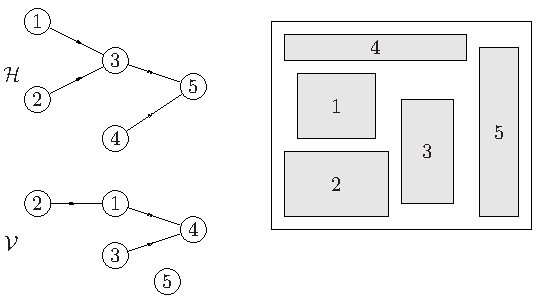
\includegraphics[width=.7\textwidth]{figures/ch08-455.pdf}
\caption*{图8.19 用水平图 $\mathcal H$、竖直图 $\mathcal V$ 规定单元相对位置的例子。若 $\mathcal H$ 中存在从 $i$ 到 $j$ 的路径，单元 $i$ 必须位于单元 $j$ 左侧；若 $\mathcal V$ 中存在从 $i$ 到 $j$ 的路径，单元 $i$ 必须位于单元 $j$ 下方。右侧布局满足两图规定的相对位置。}
\end{figure}
规定竖直相对位置的最小不等式组为
\[y_2\geq0,\quad y_3\geq0,\quad y_5\geq0,\quad y_4+h_4\leq H,\quad y_5+h_5\leq H,\]
\[y_2+h_2\leq y_1,\qquad y_1+h_1\leq y_4,\qquad y_3+h_3\leq y_4.\]
\subsection{通过凸优化进行平面布局}
本模型的变量为外包盒宽、高 $W,H$，以及单元的宽、高和位置 $w_i,h_i,x_i,w_i$，$i=1,\ldots,N$。施加外包盒约束(8.35)和相对位置约束(8.34)，它们都是线性不等式。目标取外包盒周长 $2(W+H)$，是变量的线性函数。下面列出一些能够表示成关于变量的凸不等式或线性等式的约束。
\subsubsection*{最小间距}
将相对位置约束 $x_i+w_i\leq x_j$，$(i,j)\in\mathcal H$，改为 $x_i+w_i+\rho\leq x_j$，并对竖直图作同样处理，就能规定单元间的最小间距 $\rho>0$。可以给两个图中每条边指定不同的最小间距。另一种选择是固定 $W,H$，以最大化最小间距 $\rho$ 为目标。
% Source PDF page 456 (printed p. 442)
\subsubsection*{单元最小面积}
为每个单元指定最小面积，即要求 $w_ih_i\geq A_i$，$A_i>0$。这些约束有多种凸不等式表示，例如 $w_i\geq A_i/h_i$、$(w_ih_i)^{1/2}\geq A_i^{1/2}$，或 $\log w_i+\log h_i\geq\log A_i$。
\subsubsection*{长宽比约束}
可以规定每个单元长宽比的上下界：
\[l_i\leq h_i/w_i\leq u_i.\]
两边乘以 $w_i$，即可化为线性不等式。也可以固定单元长宽比，此时得到线性等式约束。
\subsubsection*{对齐约束}
可以要求两个单元的某条边或中心线对齐。例如，单元 $i$ 的水平中心线与单元 $j$ 顶边对齐时，
\[y_i+h_i/2=y_j+h_j.\]
这些是线性等式约束。也可以同样要求单元紧贴外包盒边界。
\subsubsection*{对称约束}
可以要求成对单元关于某条竖直轴或水平轴对称，轴可以固定或浮动，即位置给定或未给定。例如，要求单元 $i,j$ 关于竖直轴 $x=x_{\mathrm{axis}}$ 对称，可施加线性等式
\[x_{\mathrm{axis}}-(x_i+w_i/2)=x_j+w_j/2-x_{\mathrm{axis}}.\]
加入这些等式，并将 $x_{\mathrm{axis}}$ 作为新变量，就能要求多对单元关于某条未指定的竖直轴对称。
\subsubsection*{相似约束}
用等式 $w_i=aw_j$、$h_i=ah_j$，可要求单元 $i$ 是单元 $j$ 缩放 $a$ 倍再平移后的结果。这里缩放因子 $a$ 必须固定。只施加其中一条约束，就要求一个单元的宽或高为另一个的给定倍数。
\subsubsection*{包含约束}
可以要求某个单元包含给定点，这施加两条线性不等式；也可以要求单元位于给定多面体内，同样通过线性不等式实现。
% Source PDF page 457 (printed p. 443)
\subsubsection*{距离约束}
可以施加各种约束，限制单元对之间的距离。最简单的是限制单元 $i,j$ 中心点之间的距离，也可以是单元上的其他固定点，例如左下角。限制两中心的距离，可用凸不等式
\[\norm{(x_i+w_i/2,y_i+h_i/2)-(x_j+w_j/2,y_j+h_j/2)}\leq D_{ij}.\]
如同布置问题，也可以限制距离之和，或以距离之和作为目标。

还可以限制单元 $i,j$ 之间的距离 $\dist(C_i,C_j)$，即各单元中一点之间的最小距离。一般可如下处理。为限制范数 $\norm{\cdot}$ 下的距离，引入四个新变量 $u_i,v_i,u_j,v_j$。坐标对 $(u_i,v_i)$ 表示 $C_i$ 中一点，$(u_j,v_j)$ 表示 $C_j$ 中一点，为此施加线性不等式
\[x_i\leq u_i\leq x_i+w_i,\qquad y_i\leq v_i\leq y_i+h_i,\]
并对单元 $j$ 作同样处理。最后，加入凸不等式
\[\norm{(u_i,v_i)-(u_j,v_j)}\leq D_{ij}\]
限制 $\dist(C_i,C_j)$。

在许多特殊情况下，可以利用相对位置约束，或导出更显式的模型，更高效地表示距离约束。例如，考虑 $\ell_\infty$ 范数，并假设相对位置约束规定单元 $i$ 在单元 $j$ 左侧。两单元的水平间距为 $x_j-(x_i+w_i)$。此时 $\dist(C_i,C_j)\leq D_{ij}$ 当且仅当
\[x_j-(x_i+w_i)\leq D_{ij},\quad y_j-(y_i+h_i)\leq D_{ij},\quad
 y_i-(y_j+h_j)\leq D_{ij}.\]
第一个不等式说明，单元 $i$ 右边与单元 $j$ 左边的水平间距不超过 $D_{ij}$；第二个说明，单元 $j$ 底边高出单元 $i$ 顶边不超过 $D_{ij}$；第三个说明，单元 $i$ 底边高出单元 $j$ 顶边不超过 $D_{ij}$。三者合起来等价于 $\dist(C_i,C_j)\leq D_{ij}$，无须引入新变量。

可以同样限制两个单元的 $\ell_1$ 或 $\ell_2$ 距离。引入新变量 $d_v$，作为单元间竖直间距的上界。限制 $\ell_1$ 距离时加入
\[y_j-(y_i+h_i)\leq d_v,\qquad y_i-(y_j+h_j)\leq d_v,\qquad d_v\geq0,\]
以及
\[x_j-(x_i+w_i)+d_v\leq D_{ij}.\]
第一项是水平间距，第二项是竖直间距上界。限制欧氏距离时，将最后一条替换为
\[(x_j-(x_i+w_i))^2+d_v^2\leq D_{ij}^2.\]
% Source PDF page 458 (printed p. 444)
\begin{figure}[htbp]\centering
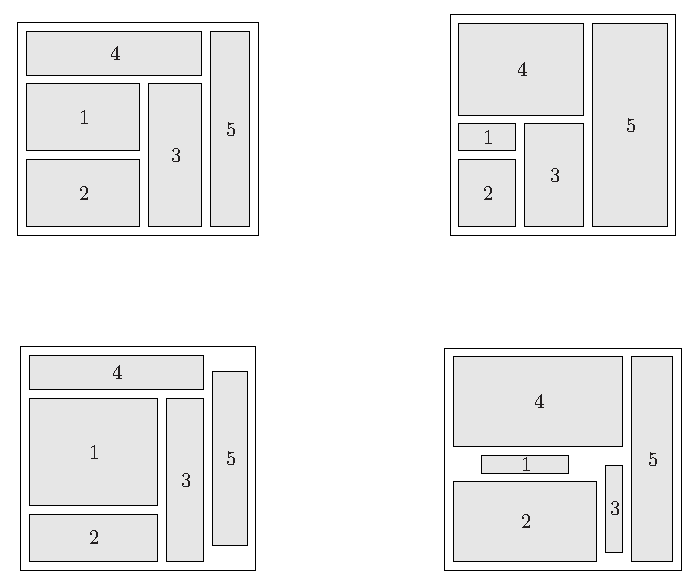
\includegraphics[width=.8\textwidth]{figures/ch08-458.pdf}
\caption*{图8.20 四个最优平面布局实例，采用图8.19的相对位置约束。每个实例都以周长最小为目标，单元之间采用相同最小间距约束，并要求长宽比在 $1/5$ 与5之间。四个实例的差别在于各单元的最小面积要求，但最小面积之和相同。}
\end{figure}
\begin{origexample}{8.7}
图8.20给出5个单元的例子，采用图8.19的顺序约束，以及四组不同约束。每例都施加相同的最小间距要求及相同长宽比约束 $1/5\leq w_i/h_i\leq5$。四例的差别在于各单元最小面积 $A_i$ 不同。选择 $A_i$ 时，使每例总最小面积要求 $\sum_{i=1}^5A_i$ 相同。
\end{origexample}
\subsection{通过几何规划进行平面布局}
平面布局问题也可以写成关于变量 $x_i,y_i,w_i,h_i,W,H$ 的几何规划。这种模型可处理的目标与约束，与凸模型略有不同。

首先，外包盒约束(8.35)与相对位置约束(8.34)都是正项式不等式，因为左端是变量之和，右端是单个变量，因而为单项式。
% Source PDF page 459 (printed p. 445)
将这些不等式除以右端，就得到标准正项式不等式。

在几何规划模型中，可以最小化外包盒面积，因为 $WH$ 为单项式，因而也是正项式。也可以精确指定每个单元面积，因为 $w_ih_i=A_i$ 是单项式等式约束。另一方面，几何规划模型不能处理对齐、对称和距离约束；但可以处理相似约束，而且可以要求单元相似而不指定缩放比例，将其作为另一个变量即可。
% Source PDF page 460 (printed p. 446)
\section*{文献说明}
\addcontentsline{toc}{section}{文献说明}
8.3.3节的欧氏距离矩阵刻画见 Schoenberg [Sch35]，也见 Gower [Gow85]。

本书沿用 Grötschel、Lovász 和 Schrijver [GLS88，第69页] 的 Löwner--John 椭球称谓。8.4节椭球近似的效率结论由 John [Joh85] 证明。Boyd、El Ghaoui、Feron 和 Balakrishnan [BEFB94，第3.7节] 针对由椭球的并、交或和定义的集合，给出几种椭球近似问题的凸模型。

8.5节的不同中心用于设计中心化，例如 Seifi、Ponnambalan 和 Vlach [SPV99]，以及割平面方法，参见 Elzinga 和 Moore [EM75]、Tarasov、Khachiyan 和 Èrlikh [TKE88]、Ye [Ye97，第8章]。由对数障碍 Hessian 定义的内椭球（原书第420页）有时称为 Dikin 椭球，是 Dikin 线性规划与二次规划算法的基础 [Dik67]。解析中心处外椭球的表达式由 Sonnevend [Son86] 给出。向非多面体凸集的推广，见 Boyd 和 El Ghaoui [BE93]、Jarre [Jar94]，以及 Nesterov 和 Nemirovski [NN94，第34页]。

自20世纪60年代起，凸优化就用于线性与非线性判别，见 Mangasarian [Man65] 和 Rosen [Ros65]。模式分类的标准教材包括 Duda、Hart 和 Stork [DHS99]，以及 Hastie、Tibshirani 和 Friedman [HTF01]。支持向量分类器的详细讨论，见 Vapnik [Vap00] 或 Schölkopf 和 Smola [SS01]。

例8.4的 Weber 点以 Weber [Web71] 命名。线性与二次布置用于电路设计，见 Kleinhaus、Sigl、Johannes 和 Antreich [KSJA91, SDJ91]。Sherwani [She99] 是近年来对 VLSI 电路设计中的布置、布局、平面规划及其他几何优化算法的综述。
% Source PDF page 461 (printed p. 447)
\section*{习题}
\addcontentsline{toc}{section}{习题}
\subsection*{在集合上的投影}
\paragraph{8.1}\textit{投影的唯一性。}证明，若 $C\subseteq\R^n$ 非空、闭且凸，范数 $\norm{\cdot}$ 严格凸，则对每个 $x_0$，都恰好存在一个离它最近的 $x\in C$。换句话说，$x_0$ 在 $C$ 上的投影唯一。
\paragraph{8.2}[Web94, Val64] \textit{凸性的 Chebyshev 刻画。}若对每个 $x_0\in\R^n$，集合 $C\in\R^n$ 中都存在唯一离 $x_0$ 最近的点，距离采用欧氏范数，则称 $C$ 为 Chebyshev 集。根据习题8.1，每个非空闭凸集都是 Chebyshev 集。本题证明逆命题，即 Motzkin 定理。

设 $C\in\R^n$ 为 Chebyshev 集。
\begin{enumerate}[label=(\alph*)]
\item 证明 $C$ 非空且闭。
\item 证明在 $C$ 上的欧氏投影 $P_C$ 连续。
\item 设 $x_0\notin C$。证明，对所有 $x=\theta x_0+(1-\theta)P_C(x_0)$、$0\leq\theta\leq1$，有 $P_C(x)=P_C(x_0)$。
\item 设 $x_0\notin C$。证明，对所有 $x=\theta x_0+(1-\theta)P_C(x_0)$、$\theta\geq1$，有 $P_C(x)=P_C(x_0)$。
\item 合并(c)与(d)，可知以 $P_C(x_0)$ 为起点、方向为 $x_0-P_C(x_0)$ 的射线上，所有点的投影都是 $P_C(x_0)$。证明这意味着 $C$ 凸。
\end{enumerate}
\paragraph{8.3}\textit{在正常锥上的欧氏投影。}
\begin{enumerate}[label=(\alph*)]
\item \textit{非负正交象限。}证明在非负正交象限上的欧氏投影由原书第399页的表达式给出。
\item \textit{半正定锥。}证明在半正定锥上的欧氏投影由原书第399页的表达式给出。
\item \textit{二阶锥。}证明 $(x_0,t_0)$ 在二阶锥
\[K=\{(x,t)\in\R^{n+1}\mid\norm x_2\leq t\}\]
上的欧氏投影为
\[P_K(x_0,t_0)=\begin{cases}
0,&\norm{x_0}_2\leq-t_0,\\
(x_0,t_0),&\norm{x_0}_2\leq t_0,\\
\tfrac12(1+t_0/\norm{x_0}_2)(x_0,\norm{x_0}_2),&\norm{x_0}_2\geq|t_0|.
\end{cases}\]
\end{enumerate}
\paragraph{8.4}点在凸集上的欧氏投影，给出一个简单的分离超平面：
\[(P_C(x_0)-x_0)^\T\bigl(x-\tfrac12(x_0+P_C(x_0))\bigr)=0.\]
找出反例，说明这个构造对一般范数不成立。
\paragraph{8.5}[HUL93，第1卷，第154页] \textit{深度函数与到边界的有符号距离。}设 $C\subseteq\R^n$ 为非空凸集，$\dist(x,C)$ 为点 $x$ 在某范数下到 $C$ 的距离。已知 $\dist(x,C)$ 关于 $x$ 凸。
\begin{enumerate}[label=(\alph*)]
\item 证明深度函数
\[\operatorname{depth}(x,C)=\dist(x,\R^n\setminus C)\]
在 $x\in C$ 时凹。
\item 到 $C$ 边界的有符号距离定义为
\[s(x)=\begin{cases}\dist(x,C),&x\notin C,\\-\operatorname{depth}(x,C),&x\in C.\end{cases}\]
因此，$s(x)$ 在 $C$ 外为正，边界上为零，内部为负。证明 $s$ 为凸函数。
\end{enumerate}
% Source PDF page 462 (printed p. 448)
\subsection*{集合之间的距离}
\paragraph{8.6}设 $C,D$ 为凸集。
\begin{enumerate}[label=(\alph*)]
\item 证明 $\dist(C,x+D)$ 关于 $x$ 凸。
\item 证明 $\dist(tC,x+tD)$ 在 $t>0$ 时关于 $(x,t)$ 凸。
\end{enumerate}
\paragraph{8.7}\textit{椭球的分离。}设两个椭球定义为
\[\mathcal E_1=\{x\mid(x-x_1)^\T P_1^{-1}(x-x_1)\leq1\},\qquad
 \mathcal E_2=\{x\mid(x-x_2)^\T P_2^{-1}(x-x_2)\leq1\},\]
其中 $P_1,P_2\in\mathbb S_{++}^n$。证明，$\mathcal E_1\cap\mathcal E_2=\varnothing$ 当且仅当存在 $a\in\R^n$ 使
\[\norm{P_1^{1/2}a}_2+\norm{P_2^{1/2}a}_2<a^\T(x_1-x_2).\]
\paragraph{8.8}\textit{多面体的相交与包含。}设两个多面体定义为
\[P_1=\{x\mid Ax\preceq b\},\qquad P_2=\{x\mid Fx\preceq g\},\]
其中 $A\in\R^{m\times n}$、$b\in\R^m$、$F\in\R^{p\times n}$、$g\in\R^p$。说明如何通过求解一个或数量不多的 LP 可行性问题完成以下任务。
\begin{enumerate}[label=(\alph*)]
\item 找到交集 $P_1\cap P_2$ 中的一点。
\item 判断是否 $P_1\subseteq P_2$。
\end{enumerate}
对以下方式定义的两个多面体重复上述问题：
\[P_1=\conv\{v_1,\ldots,v_K\},\qquad P_2=\conv\{w_1,\ldots,w_L\},\]
其中 $v_1,\ldots,v_K,w_1,\ldots,w_L\in\R^n$。
\subsection*{欧氏距离与角度问题}
\paragraph{8.9}\textit{与给定数据最近的欧氏距离矩阵。}给定数据 $\widehat d_{ij}$、$i,j=1,\ldots,n$，它们是 $\R^k$ 中向量间欧氏距离受到干扰的测量值：
\[\widehat d_{ij}=\norm{x_i-x_j}_2+v_{ij},\qquad i,j=1,\ldots,n,\]
其中 $v_{ij}$ 为噪声或误差。对所有 $i,j$，数据满足 $\widehat d_{ij}\geq0$、$\widehat d_{ij}=\widehat d_{ji}$。维数 $k$ 未指定。

说明如何用凸优化求解：寻找维数 $k$ 及 $x_1,\ldots,x_n\in\R^k$，使 $\sum_{i,j=1}^n(d_{ij}-\widehat d_{ij})^2$ 最小，其中 $d_{ij}=\norm{x_i-x_j}_2$。换句话说，给定近似欧氏距离的数据，寻找最小二乘意义下最接近它们的一组真实欧氏距离。
\paragraph{8.10}\textit{极小极大角度拟合。}设 $y_1,\ldots,y_m\in\R^k$ 为变量 $x\in\R^n$ 的仿射函数：
\[y_i=A_ix+b_i,\qquad i=1,\ldots,m,\]
$z_1,\ldots,z_m\in\R^k$ 为给定非零向量。希望选择满足某些凸约束，例如线性不等式的 $x$，使 $y_i$ 与 $z_i$ 之间的最大夹角
\[\max\{\angle(y_1,z_1),\ldots,\angle(y_m,z_m)\}\]
最小。非零向量间角度按通常方式定义：
\[\angle(u,v)=\cos^{-1}\left(\frac{u^\T v}{\norm u_2\norm v_2}\right),\]
其中 $\cos^{-1}(a)\in[0,\pi]$。只关心最优目标值不超过 $\pi/2$ 的情况。

将此问题写成凸或拟凸优化问题。当 $x$ 的约束是线性不等式时，需要求解哪类问题？
% Source PDF page 463 (printed p. 449)
\paragraph{8.11}\textit{包含给定点的最小欧氏锥。}在 $\R^n$ 中，中心方向 $c\ne0$、角半径 $0\leq\theta\leq\pi/2$ 的欧氏锥定义为
\[\{x\in\R^n\mid\angle(c,x)\leq\theta\}.\]
欧氏锥是二阶锥，即能表示为二阶锥在非奇异线性映射下的像。

设 $a_1,\ldots,a_m\in\R^n$。怎样找到包含这些点、角半径最小的欧氏锥？特别地，应说明如何求解可行性问题，即判断是否存在包含这些点的欧氏锥。
\subsection*{极值体积椭球}
\paragraph{8.12}证明，内接于一个集合的最大体积椭球唯一。证明，一个集合的 Löwner--John 椭球唯一。
\paragraph{8.13}\textit{单纯形的 Löwner--John 椭球。}本题证明，$\R^n$ 中单纯形的 Löwner--John 椭球，必须缩小 $n$ 倍才能放入该单纯形内。由于 Löwner--John 椭球具有仿射不变性，只需对一个特定单纯形证明。

求单纯形 $C=\conv\{0,e_1,\ldots,e_n\}$ 的 Löwner--John 椭球 $\mathcal E_{\mathrm{lj}}$。证明，$\mathcal E_{\mathrm{lj}}$ 必须按因子 $1/n$ 缩小，才能放入单纯形内。
\paragraph{8.14}\textit{椭球内近似的效率。}设 $C$ 为 $\R^n$ 中多面体，$C=\{x\mid Ax\preceq b\}$，且 $\{x\mid Ax\prec b\}$ 非空。
\begin{enumerate}[label=(\alph*)]
\item 证明，内接于 $C$ 的最大体积椭球，围绕中心扩大 $n$ 倍后，得到包含 $C$ 的椭球。
\item 证明，若 $C$ 关于原点对称，即具有形式 $C=\{x\mid-\one\preceq Ax\preceq\one\}$，则将最大体积内接椭球扩大 $\sqrt n$ 倍，就得到包含 $C$ 的椭球。
\end{enumerate}
\paragraph{8.15}\textit{覆盖椭球并集的最小体积椭球。}将以下问题写成凸优化：寻找包含 $K$ 个给定椭球
\[\mathcal E_i=\{x\mid x^\T A_ix+2b_i^\T x+c_i\leq0\},\quad i=1,\ldots,K\]
的最小体积椭球 $\mathcal E=\{x\mid(x-x_0)^\T A^{-1}(x-x_0)\leq1\}$。
\textit{提示：}见附录B。
\paragraph{8.16}\textit{多面体内的最大体积矩形。}将以下问题写成凸优化：寻找位于多面体 $P=\{x\mid Ax\preceq b\}$ 内、体积最大的矩形
\[R=\{x\in\R^n\mid l\preceq x\preceq u\}.\]
变量为 $l,u\in\R^n$。所建模型不应包含指数数量的约束。
\subsection*{求中心}
\paragraph{8.17}\textit{解析中心的仿射不变性。}证明，不等式组的解析中心具有仿射不变性。证明，它在不等式正数缩放下保持不变。
\paragraph{8.18}\textit{解析中心与冗余不等式。}描述同一个多面体的两组线性不等式，可能具有不同解析中心。证明，通过加入冗余不等式，可以使多面体
\[P=\{x\in\R^n\mid Ax\preceq b\}\]
的任意内点 $x_0$ 成为解析中心。
% Source PDF page 464 (printed p. 450)
具体地，设 $A\in\R^{m\times n}$、$Ax_0\prec b$。证明，存在 $c\in\R^n$、$\gamma\in\R$ 以及正整数 $q$，使 $P$ 是如下 $m+q$ 个不等式的解集：
\begin{equation}Ax\preceq b,\qquad c^\T x\leq\gamma,\qquad c^\T x\leq\gamma,\quad\ldots,\quad c^\T x\leq\gamma,\tag{8.36}\end{equation}
其中不等式 $c^\T x\leq\gamma$ 添加 $q$ 次，并且 $x_0$ 是式(8.36)的解析中心。
\paragraph{8.19}设 $x_{\mathrm{ac}}$ 是线性不等式组
\[a_i^\T x\leq b_i,\qquad i=1,\ldots,m\]
的解析中心，定义 $H$ 为对数障碍在 $x_{\mathrm{ac}}$ 处的 Hessian：
\[H=\sum_{i=1}^m\frac1{(b_i-a_i^\T x_{\mathrm{ac}})^2}a_ia_i^\T.\]
证明，若
\[b_k-a_k^\T x_{\mathrm{ac}}\geq m(a_k^\T H^{-1}a_k)^{1/2},\]
则第 $k$ 条不等式冗余，即删去它不会改变可行集。
\paragraph{8.20}\textit{由线性矩阵不等式解析中心得到的椭球近似。}设 $C$ 为 LMI
\[x_1A_1+x_2A_2+\cdots+x_nA_n\preceq B\]
的解集，$A_i,B\in\mathbb S^m$，$x_{\mathrm{ac}}$ 为其解析中心。证明
\[\mathcal E_{\mathrm{inner}}\subseteq C\subseteq\mathcal E_{\mathrm{outer}},\]
其中
\[\mathcal E_{\mathrm{inner}}=\{x\mid(x-x_{\mathrm{ac}})^\T H(x-x_{\mathrm{ac}})\leq1\},\]
\[\mathcal E_{\mathrm{outer}}=\{x\mid(x-x_{\mathrm{ac}})^\T H(x-x_{\mathrm{ac}})\leq m(m-1)\},\]
$H$ 是对数障碍
\[-\log\det(B-x_1A_1-x_2A_2-\cdots-x_nA_n)\]
在 $x_{\mathrm{ac}}$ 处的 Hessian。
\paragraph{8.21}[BYT99] \textit{解析中心的最大似然解释。}采用原书第352页的线性测量模型
\[y=Ax+v,\]
其中 $A\in\R^{m\times n}$。假设噪声分量 $v_i$ 独立同分布，支撑为 $[-1,1]$。与测量 $y\in\R^m$ 一致的参数 $x$ 构成由线性不等式
\begin{equation}-\one+y\preceq Ax\preceq\one+y\tag{8.37}\end{equation}
定义的多面体。设 $v_i$ 的概率密度为
\[p(v)=\begin{cases}\alpha_r(1-v^2)^r,&-1\leq v\leq1,\\0,&\text{其他情况},\end{cases}\]
其中 $r\geq1$、$\alpha_r>0$。证明，$x$ 的最大似然估计为式(8.37)的解析中心。
\paragraph{8.22}\textit{重心。}内部非空的集合 $C\subseteq\R^n$ 的重心定义为
\[x_{\mathrm{cg}}=\frac{\int_C u\,du}{\int_C1\,du}.\]
% Source PDF page 465 (printed p. 451)
重心具有仿射不变性，而且显然取决于集合 $C$ 本身，而不是它的具体描述。不过，与本章介绍的其他中心不同，除椭球、球、单纯形等简单情况外，计算重心非常困难。

证明，重心 $x_{\mathrm{cg}}$ 是凸函数
\[f(x)=\int_C\norm{u-x}_2^2\,du\]
的最小点。
\subsection*{分类}
\paragraph{8.23}\textit{稳健线性判别。}考虑式(8.23)的稳健线性判别问题。
\begin{enumerate}[label=(\alph*)]
\item 证明，最优值 $t^\star$ 为正，当且仅当两组点可线性分离。在可线性分离时，证明最优 $a^\star$ 使 $\norm a_2\leq1$ 取等号，即 $\norm{a^\star}_2=1$。
\item 用换元 $\widetilde a=a/t$、$\widetilde b=b/t$ 证明问题(8.23)等价于 QP
\[\begin{array}{ll}
\text{最小化}&\norm{\widetilde a}_2\\
\text{约束为}&\widetilde a^\T x_i-\widetilde b\geq1,\quad i=1,\ldots,N,\\
&\widetilde a^\T y_i-\widetilde b\leq-1,\quad i=1,\ldots,M.
\end{array}\]
\end{enumerate}
\paragraph{8.24}\textit{对权重误差具有最大稳健性的线性判别。}给定 $\R^n$ 中可线性分离的两组点 $\{x_1,\ldots,x_N\}$、$\{y_1,\ldots,y_M\}$。8.6.1节介绍了怎样寻找既判别二者、又使函数值间隔最大的仿射函数。还可以考虑向量 $a$ 变化时的稳健性，$a$ 有时称为权重向量。给定使 $f(x)=a^\T x-b$ 分离两组点的 $a,b$，将权重误差裕量定义为使仿射函数 $(a+u)^\T x-b$ 不再分离两组点的最小 $u\in\R^n$ 的范数。换句话说，权重误差裕量为最大的 $\rho$，使
\[(a+u)^\T x_i\geq b,\quad i=1,\ldots,N,\qquad
 (a+u)^\T y_j\leq b,\quad i=1,\ldots,M\]
对所有 $\norm u_2\leq\rho$ 都成立。

说明如何在归一化约束 $\norm a_2\leq1$ 下，求使权重误差裕量最大的 $a,b$。
\paragraph{8.25}\textit{最接近球形的分离椭球。}给定两组向量 $x_1,\ldots,x_N\in\R^n$、$y_1,\ldots,y_M\in\R^n$，希望寻找偏心程度最小，即定义矩阵条件数最小，的椭球 $\mathcal E$，满足 $x_i\in\mathcal E$、$i=1,\ldots,N$，以及 $y_i\notin\operatorname{int}\mathcal E$、$i=1,\ldots,M$。将它写成凸优化问题。
\subsection*{布置与平面布局}
\paragraph{8.26}\textit{二次布置。}考虑 $\R^2$ 中由含 $N$ 个节点的无向图 $\mathcal A$ 定义的布置问题，代价为二次：
\[\text{最小化}\quad\sum_{(i,j)\in\mathcal A}\norm{x_i-x_j}_2^2.\]
变量为位置 $x_i\in\R^2$、$i=1,\ldots,M$；位置 $x_i$、$i=M+1,\ldots,N$ 已给定。定义 $u,v\in\R^M$ 为
\[u=(x_{11},x_{21},\ldots,x_{M1}),\qquad
 v=(x_{12},x_{22},\ldots,x_{M2}),\]
分别包含自由节点的第一、第二分量。
% Source PDF page 466 (printed p. 452)
证明，可通过求解两组线性方程
\[Cu=d_1,\qquad Cv=d_2\]
得到 $u,v$，其中 $C\in\mathbb S^M$。用图 $\mathcal A$ 给出 $C$ 的各系数的简单表达式。
\paragraph{8.27}\textit{带最小距离约束的问题。}考虑以 $x_1,\ldots,x_N\in\R^k$ 为变量的问题。目标 $f_0(x_1,\ldots,x_N)$ 凸，约束
\[f_i(x_1,\ldots,x_N)\leq0,\qquad i=1,\ldots,m\]
凸，即各 $f_i:\R^{Nk}\to\R$ 凸。此外有最小距离约束
\[\norm{x_i-x_j}_2\geq D_{\min},\quad i\ne j,\quad i,j=1,\ldots,N.\]
这一般是困难的非凸问题。

按照平面布局中的做法，可以构造凸的限制问题：它是凸问题，但可行集更小。求解限制问题容易，而且其任意解保证是原非凸问题的可行解。设 $a_{ij}\in\R^k$、$i<j$、$i,j=1,\ldots,N$ 满足 $\norm{a_{ij}}_2=1$。证明，限制问题
\[\begin{array}{ll}
\text{最小化}&f_0(x_1,\ldots,x_N)\\
\text{约束为}&f_i(x_1,\ldots,x_N)\leq0,\quad i=1,\ldots,m,\\
&a_{ij}^\T(x_i-x_j)\geq D_{\min},\quad i<j,\quad i,j=1,\ldots,N,
\end{array}\]
凸，并且任意可行点均满足最小距离约束。

\textit{注：}选择方向 $a_{ij}$ 有许多好的启发式方法。一种简单方法从近似解 $\widehat x_1,\ldots,\widehat x_N$ 出发，它不必满足最小距离约束，再取 $a_{ij}=(\widehat x_i-\widehat x_j)/\norm{\widehat x_i-\widehat x_j}_2$。
\subsection*{其他问题}
\paragraph{8.28}设两个多面体描述为
\[P_1=\{x\mid Ax\preceq b\},\qquad
 P_2=\{x\mid-\one\preceq Cx\preceq\one\},\]
其中 $A\in\R^{m\times n}$、$C\in\R^{p\times n}$、$b\in\R^m$。多面体 $P_2$ 关于原点对称。对 $t\geq0$、$x_c\in\R^n$，记
\[tP_2+x_c=\{tx+x_c\mid x\in P_2\},\]
即先将 $P_2$ 关于原点缩放 $t$ 倍，再将中心平移到 $x_c$ 后得到的多面体。

说明如何用一个 LP 或一组 LP 求解以下问题。
\begin{enumerate}[label=(\alph*)]
\item 寻找位于 $P_1$ 内的最大多面体 $tP_2+x_c$，即
\[\begin{array}{ll}\text{最大化}&t\\\text{约束为}&tP_2+x_c\subseteq P_1,\\&t\geq0.\end{array}\]
\item 寻找包含 $P_1$ 的最小多面体 $tP_2+x_c$，即
\[\begin{array}{ll}\text{最小化}&t\\\text{约束为}&P_1\subseteq tP_2+x_c,\\&t\geq0.\end{array}\]
\end{enumerate}
% Source PDF page 467 (printed p. 453)
两个问题的变量均为 $t\in\R$、$x_c\in\R^n$。
\paragraph{8.29}\textit{多面体外近似。}设 $P=\{x\in\R^n\mid Ax\preceq b\}$ 为多面体，$C\subseteq\R^n$ 为给定集合，不必凸。利用支撑函数 $S_C$，将以下问题写成 LP：
\[\begin{array}{ll}\text{最小化}&t\\\text{约束为}&C\subseteq tP+x,\\&t\geq0.\end{array}\]
这里 $tP+x=\{tu+x\mid u\in P\}$，是 $P$ 关于原点缩放 $t$ 倍再平移 $x$ 后的多面体。变量为 $t\in\R$、$x\in\R^n$。
\paragraph{8.30}\textit{分段圆弧曲线插值。}给定点列 $a_1,\ldots,a_n\in\R^2$。构造依次通过这些点的曲线，相邻两点间为圆弧，即圆的一部分，或线段，将线段视作半径无穷大的圆弧。有许多圆弧连接 $a_i,a_{i+1}$，用圆弧在 $a_i$ 处切线与线段 $[a_i,a_{i+1}]$ 的夹角 $\theta_i\in(-\pi,\pi)$ 参数化。因此，$\theta_i=0$ 意味着两点间圆弧实际上是线段；$\theta_i=\pi/2$ 意味着半圆，位于线段 $[a_1,a_2]$ 上方；$\theta_i=-\pi/2$ 意味着半圆，位于该线段下方。见下图。
\begin{center}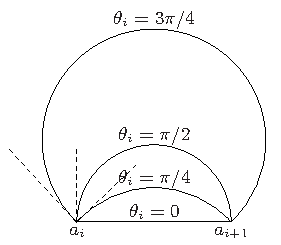
\includegraphics[width=.35\textwidth]{figures/ch08-ex467a.pdf}\end{center}
曲线由 $\theta_1,\ldots,\theta_n$ 完全指定，各角度可在 $(-\pi,\pi)$ 内选择。$\theta_i$ 的选择影响曲线的几种性质，例如总弧长 $L$，以及接点角不连续性，后者描述如下。

在每个 $a_i$、$i=2,\ldots,n-1$ 处，两段圆弧相接，一段从前一点而来，一段通向下一点。若两条切线方向恰好相反，从而曲线在 $a_i$ 处可微，则称该点没有接点角不连续。一般地，将 $a_i$ 处接点角不连续量定义为 $|\theta_{i-1}+\theta_i+\psi_i|$，其中 $\psi_i$ 为线段 $[a_i,a_{i+1}]$ 与 $[a_{i-1},a_i]$ 的夹角，即 $\psi_i=\angle(a_i-a_{i+1},a_{i-1}-a_i)$，如下图。由于各 $a_i$ 已知，角度 $\psi_i$ 也已知。
\begin{center}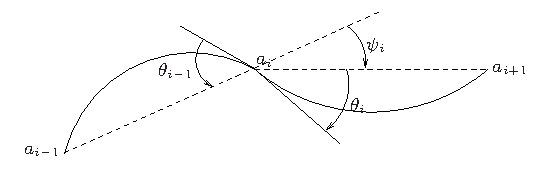
\includegraphics[width=.65\textwidth]{figures/ch08-ex467b.pdf}\end{center}
总接点角不连续量定义为
\[D=\sum_{i=2}^n|\theta_{i-1}+\theta_i+\psi_i|.\]
将最小化总弧长 $L$ 与总接点角不连续量 $D$ 的问题，写成双准则凸优化。说明如何找到最优权衡曲线上的极端点。
% Source PDF page 468 (printed p. 454): blank page in source.

